\documentclass[12pt]{report}
\usepackage[osf]{garamondx}
\usepackage[garamondx,cmbraces]{newtxmath}
\usepackage{marginnote}
\usepackage[top=2cm, bottom=2cm, outer=3cm, inner=3cm, heightrounded, 
            marginparwidth=2cm, marginparsep=0.5cm]{geometry}
\usepackage{setspace}
\usepackage[backend=biber, style=authoryear]{biblatex}
\usepackage{nicefrac}
\usepackage{amsmath}
\usepackage{algorithm}
\usepackage{algorithmicx}
\usepackage{algpseudocode}
\usepackage{hyperref}
\usepackage[acronym,nonumberlist]{glossaries}

\newcommand{\comment}[1]{\marginnote{\textit{#1}}}

\newcommand{\defn}[1]{\textit{#1}}
\newcommand{\software}[1]{\textit{#1}}
\newcommand{\etal}{\textit{et al.}}

\newcommand{\set}[1]{\left\lbrace#1\right\rbrace}
\renewcommand{\emptyset}{\varnothing}
\renewcommand{\vec}[1]{\mathbf{#1}}
\renewcommand{\star}[1]{#1^*}
\renewcommand{\d}{\mathrm{d}\,}

\DeclareMathOperator*{\argmin}{arg\,min}
\DeclareMathOperator*{\argmax}{arg\,max}

\DeclareMathOperator{\Exponential}{Exponential}
\DeclareMathOperator{\Uniform}{Uniform}
\DeclareMathOperator{\E}{E}
\DeclareMathOperator{\Var}{Var}

\DeclareMathOperator{\inc}{in}
\DeclareMathOperator{\out}{out}

\newcommand{\N}{\mathcal{N}}
\renewcommand{\L}{\mathcal{L}}

\newacronym{MCMC}{MCMC}{Markov chain Monte Carlo}
\newacronym{ER}{ER}{Erd\H{o}s-R\'enyi}
\newacronym{BA}{BA}{Barab\'asi-Albert}
\newacronym{WS}{WS}{Watts-Strogatz}
\newacronym{SI}{SI}{susceptible-infected}
\newacronym{SVM}{SVM}{support vector machine}
\newacronym{PCA}{PCA}{principal components analysis}
\newacronym{SMC}{SMC}{sequential Monte Carlo}
\newacronym{ABC}{ABC}{approximate Bayesian computation}
\newacronym{nltt}{nLTT}{normalized lineages-through-time}
\newacronym{ltt}{LTT}{lineages-through-time}
\newacronym{pdf}{pdf}{probability density function}
\newacronym{rv}{rv}{random variable}
\newacronym{ML}{ML}{maximum likelihood}
\newacronym{MAP}{MAP}{maximum \textit{a posteriori}}
\newacronym{GSL}{GSL}{GNU scientific library}
\newacronym{SIR}{SIR}{susceptible-infected-recovered}
\newacronym{IS}{IS}{importance sampling}
\newacronym{SIS}{SIS}{sequential importance sampling}
\newacronym{HMM}{HMM}{hidden Markov model}
\newacronym{iid}{i.i.d.}{independent and identically distributed}

\newglossaryentry{alpha}{
  name=$\alpha$,
  description=preferential attachment power parameter in Barab\'asi-Albert networks
}
\newglossaryentry{m}{
  name=$m$,
  description=number of edges added per vertex when constructing a Barab\'asi-Albert network
}
\newglossaryentry{N}{
  name=$N$,
  description=number of nodes in the network
}
\newglossaryentry{I}{
  name=$I$,
  description=number of nodes which are eventually infected
}
\newglossaryentry{p}{
  name=$p$,
  description=edge density parameter in Erd\H{o}s-R\'enyi networks
}
\newglossaryentry{lambda}{
  name=$\lambda$,
  description=decay factor meta-parameter for tree kernel
}
\newglossaryentry{sigma}{
  name=$\sigma$,
  description=radial basis function variance meta-parameter for tree kernel
}
\newglossaryentry{n}{
  name=$n$,
  description=number of particles used for ABC-SMC
}
\newglossaryentry{M}{
  name=$M$,
  description=number of simulated datasets per particle in ABC-SMC
}

\graphicspath{{figures/}}

\title{Phylodynamic inference of contact network parameters through approximate
Bayesian computation}
\author{Rosemary M. McCloskey and Art F.Y. Poon}

\addbibresource{papers.bib}
\makeglossaries

\frenchspacing
\onehalfspacing

\begin{document}

\maketitle

\tableofcontents

\listoffigures

\printglossary[title=List of Symbols]
\printglossary[title=List of Abbreviations,type=\acronymtype]

\chapter{Introduction}
\section{Phylogenetics and phylodynamics}
\label{sec:phylo}

\subsection{Phylogenetic trees}

In evolutionary biology, a \defn{phylogeny}, or \defn{phylogenetic tree}, is a
graphical representation of the evolutionary relationships among a group of
organisms or species (generally, \defn{taxa})~\autocite{haeckel1866generelle}.
The \defn{tips} of a phylogeny, that is, the nodes without any descendants,
correspond to \defn{extant}, or observed, taxa. The \defn{internal nodes}
correspond to their common ancestors, {\color{blue}\uline{usually extinct
(although occasionally the internal nodes may be observed as well, eg.
\autocite{jombart2011reconstructing}).}} The edges or \defn{branches} of the
phylogeny connect ancestors to their descendants. Phylogenies may have a
\defn{root}, which is a node with no descendants distinguished as the most
recent common ancestor of all the extant
taxa~\autocite{harding1971probabilities}. When such a root exists, the tree is
referred to as being \defn{rooted}; otherwise, it is \defn{unrooted}. The
structural arrangement of nodes and edges in the tree is referred to as its
\defn{topology}~\autocite{cavalli1967phylogenetic}. 

The branches of the tree may have associated lengths, representing either
evolutionary distance or calendar time between ancestors and their descendants.
The term ``evolutionary distance'' is used here imprecisely to mean any sort of
quantitative measure of evolution, such as the number of differences between
the DNA sequences of an ancestor and its descendant, or the difference in
average body mass or height. A phylogeny with branch lengths in calendar time
units is often referred to as \defn{time-scaled}. In a time-scaled phylogeny,
the internal nodes can be mapped onto a timeline by using the tips of the tree,
which usually correspond to the present day, reference
points~\autocite{nee1992tempo}. The corresponding points on the timeline are
called \defn{branching times}, and the rate of their accumulation is referred
to as the \defn{branching rate}. Rooted trees whose tips are all the same
distance from the root are called \defn{ultrametric}
trees~\autocite{buneman1974note}. These concepts are illustrated in
\cref{fig:speciestree}.

\begin{figure}[ht]
  \centering
  \includegraphics{speciestree.pdf}
  \caption[Illustration of a rooted, ultrametric, time-scaled phylogeny.]
    {Illustration of a rooted, ultrametric, time-scaled phylogeny. The tips of
      the tree, which represent extant taxa, are placed at the present day on
      the time axis. Internal nodes, representing extinct common ancestors to
      the extant taxa, fall in the past. The topology of the tree indicates
      that cats and dogs are the most closely related pair of species, whereas
      fish is most distantly related to any other taxon in the tree.}
  \label{fig:speciestree}
\end{figure}

\subsection{Transmission trees}

In epidemiology, a \defn{transmission tree} is a graphical representation of an
epidemic's progress through a population~\autocite{ypma2013relating}. Like
phylogenies, transmission trees have tips, nodes, edges, and branch lengths.
However, rather than recording an evolutionary process (speciation), they
record an epidemiological process (transmission). The tips of a transmission
tree represent the removal by sampling of infected hosts, while internal nodes
correspond to transmissions from one host to another. Transmission trees
generally have branch lengths in units of calendar time, with branching times
indicating times of transmission. The root of a transmission tree corresponds
to the initially infected patient who introduced the epidemic into the network,
also known as the \defn{index case}. The internal nodes may be labelled with
the donor of the transmission pair, if this is known. The tips of the tree,
rather than being fixed at the present day, are placed at the time at which the
individual was removed from the epidemic, such as by death, recovery,
isolation, behaviour change, or migration~\autocite{stadler2013uncovering}.
Consequently, the transmission tree may not be ultrametric, but may have tips
located at varying distances from the root. Such trees are said to have
\defn{heterochronous} taxa~\autocite{drummond2003measurably}, in contrast to
the \defn{isochronous} taxa found in most phylogenies of macro-organisms. A
transmission tree is illustrated in \cref{fig:contactnet} (right). 
The object on the right of the figure is called a \defn{contact
network}, which depicts the entire susceptible population along with all
possible routes of disease transmission. Contact networks, and their
relationships to transmission trees, will be discussed further in
\cref{sec:contactnet}.

Each infected individual in an epidemic may appear at nodes of the transmission
tree more than once. This is different from the transmission \emph{network}, in
which each infected individual appears exactly once, and edges are in
one-to-one correspondence with transmissions~\autocite{welch2011statistical,
keeling2005networks}. The distinction between the two objects is illustrated in
\cref{fig:contactnet}. However, since transmission networks generally have no
cycles (unless re-infection occurs), they are trees in the graph theoretical
sense, and hence are sometimes also referred to as transmission
trees~\autocite[\eg][]{kenah2015algorithms}. In this work, we reserve the term
``transmission tree'' for the objects depicted on the right side of
\cref{fig:contactnet}, following \eg~\autocite{stadler2013uncovering}. The term
``transmission network'' is taken to mean the subgraph of the contact network
along which transmissions occurred, following
\eg~\autocite{welch2011statistical, keeling2005networks}.

\begin{figure}
    \centering
    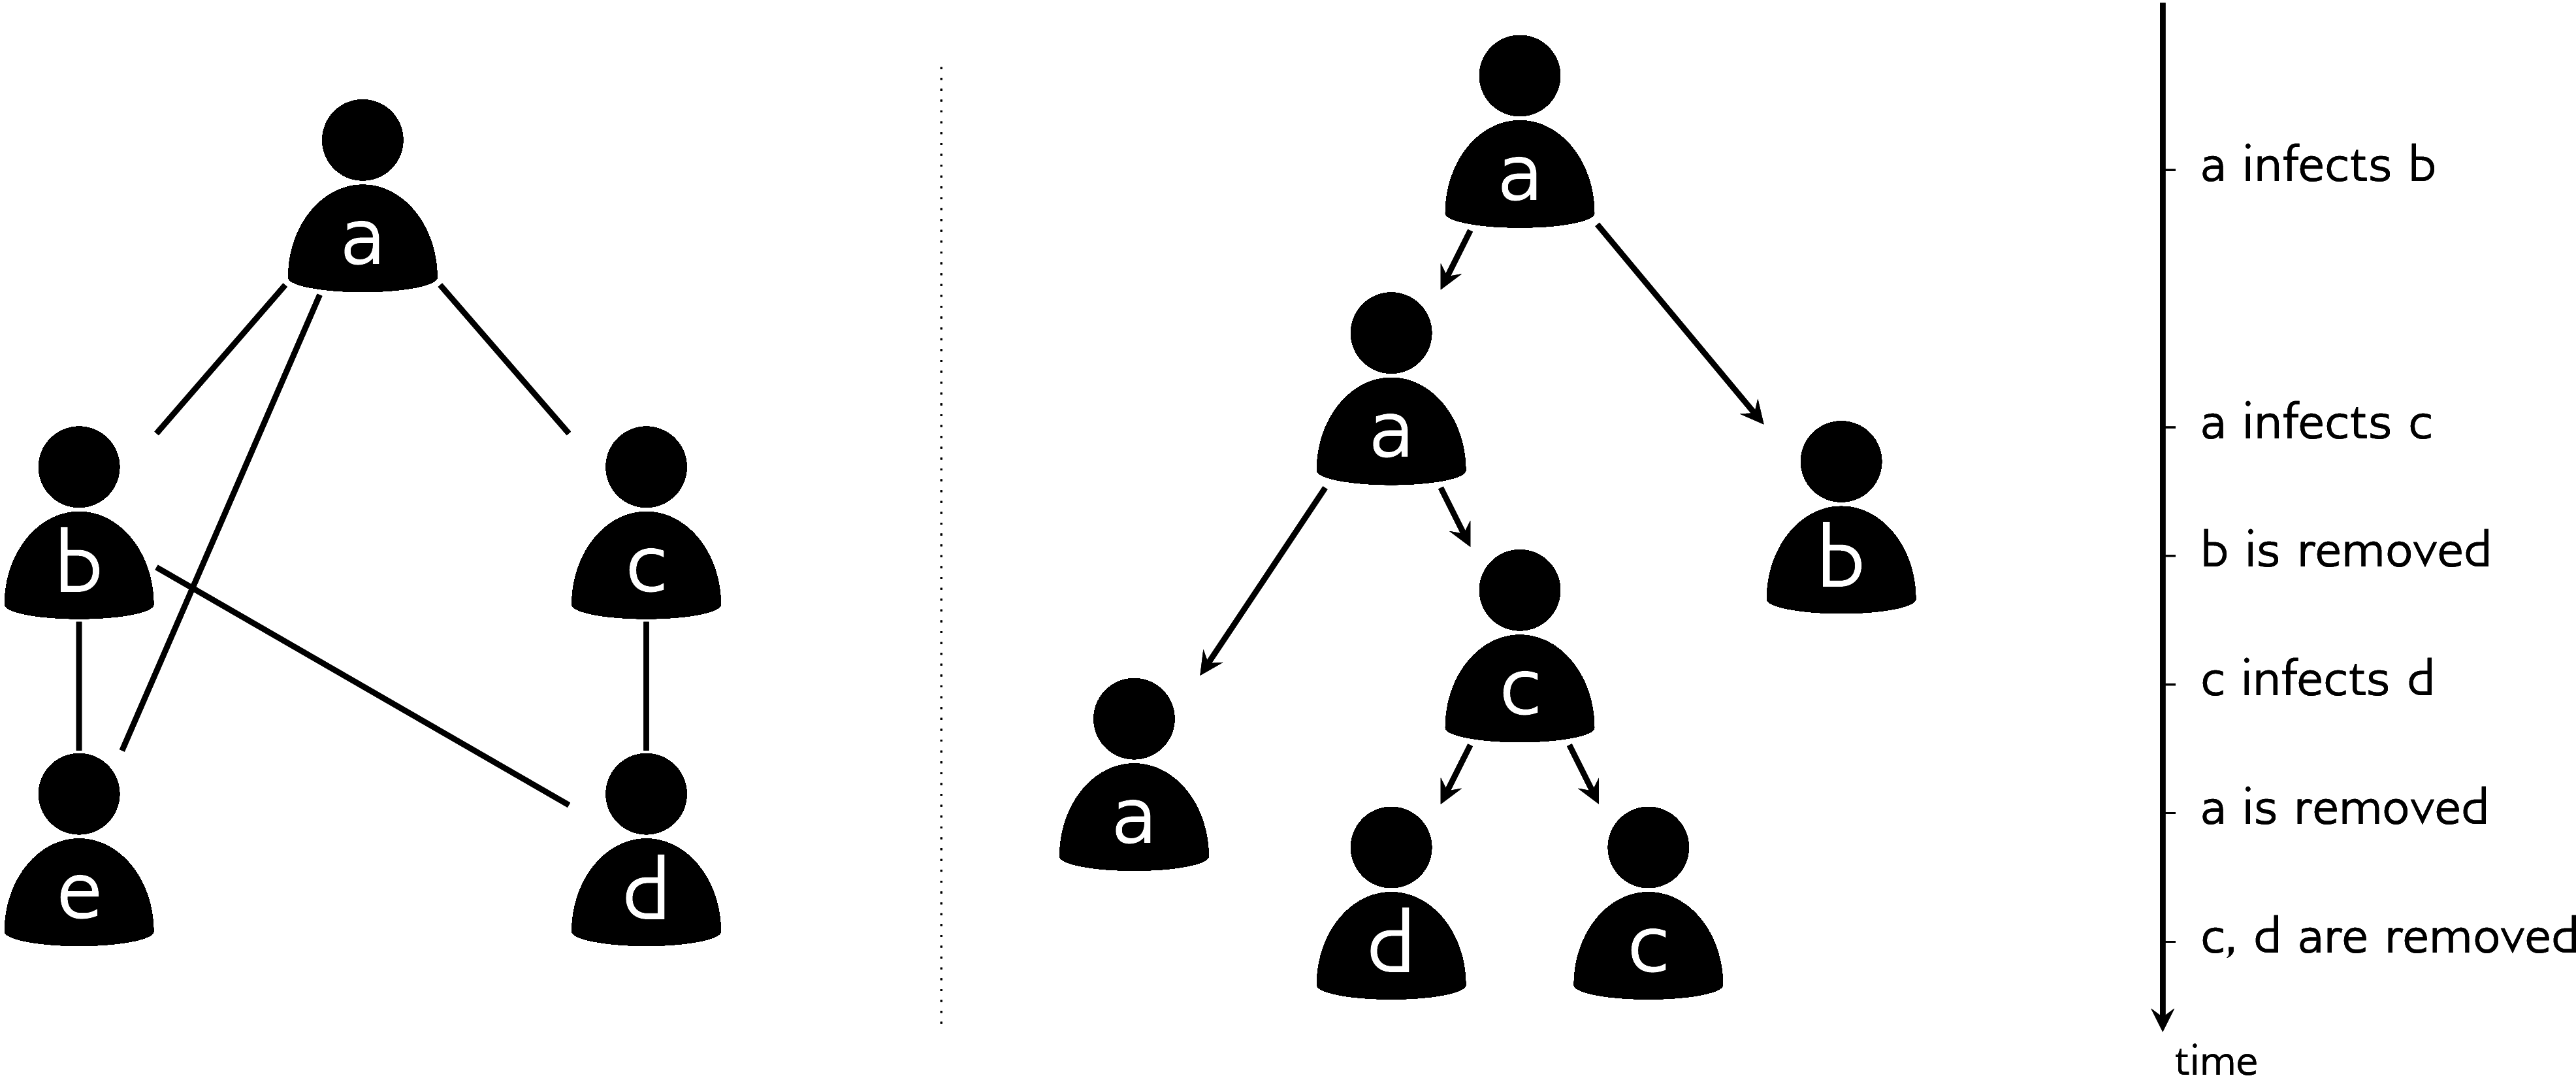
\includegraphics[width=\textwidth]{contactnet.pdf}
    \caption[Illustration of a contact network and transmission tree.]{
      Illustration of epidemic spread over a contact network, and the
      corresponding transmission tree. (Left) A contact network with five
      hosts, labelled $a$ through $e$. Thick shaded edges indicate symmetric
      contacts among the hosts. The transmission network is indicated by
      coloured arrows. The epidemic began with node $a$, who transmitted to
      nodes $b$ and $c$. Node $c$ further transmitted to node $d$. Node $e$ was
      not infected. (Right) The transmission tree corresponding to this
      scenario, with a timeline of transmission and removal times.
    }
    \label{fig:contactnet}
\end{figure}

Since transmission trees are essentially a detailed record of an epidemic's
progress, they contain substantial epidemiological information. As a basic
example, the \gls{ltt} plot~\autocite{nee1992tempo}, which plots the number of
lineages in a phylogeny against time, can be used to quantify the incidence of
new infections over the course of an epidemic~\autocite{holmes1995revealing}.
However, in all but the most well-studied of epidemics, transmission trees are
not possible to assemble through traditional epidemiological
methods~\autocite{welch2011statistical}. The time and effort to conduct
detailed interviews and contact tracing of a sufficient number of infected
individuals is usually prohibitive, and may additionally be confounded by
misreporting and other challenges~\autocite{eames2015six}. However, it turns
out that for viral epidemics, some of the epidemiological information contained
in the transmission tree leaves a mark on the viral genetic material
circulating in the population. A family of methods called
\defn{phylodynamics}~\autocite{grenfell2004unifying} addresses the challenge of
estimating epidemiological parameters from viral sequence
data~\autocite{volz2013viral}.

\subsection{Phylodynamics: linking evolution and epidemiology}
\label{subsec:phylodynamics}

%Most modern analyses use model-based methods, which simultaneously
%estimate the phylogeny with branch lengths and the parameters of a model of
%evolution. Although they usually work well in practice, the estimated topology
%can vary based on the model used and, in the case of Bayesian analysis, the
%priors. In addition, intra-host viral populations are genetically
%heterogeneous, so choosing a single representative genotype per host is
%necessarily imprecise. One can use either the genotype of a specific virion
%sampled from the host, or a synthetic genotype, such as a consensus or
%reconstructed ancestral sequence.

The basis of phylodynamics is the fact that, for RNA viruses, epidemiological
and evolutionary processes occur on similar time
scales~\autocite{drummond2003measurably}. In fact, these two processes
interact, such that it is possible to detect the influence of host epidemiology
on the evolutionary history of the virus as recorded in an \defn{inter-host
viral phylogeny}. Phylodynamic methods aim to detect and quantify the
signatures of epidemiological processes in these
phylogenies~\autocite{pybus2009evolutionary, volz2013viral}, which relate one
representative viral genotype from each host in an infected population. These
methods have been used to investigate parameters such as transmission rate,
recovery rate, and basic reproductive number~\autocite{pybus2009evolutionary,
volz2013viral}. The majority of phylodynamic studies attempt to infer the
parameters of an epidemiological model for which the likelihood of an observed
phylogeny can be calculated. Most often, this is some variation of the
birth-death~\autocite{kendall1948generalized, stadler2012estimating} or
coalescent~\autocite{kingman1982coalescent, volz2012complex} models. These
methods either assume the viral phylogeny is known, as we do in this work, or
(more commonly) integrate over phylogenetic uncertainty in a Bayesian
framework. Phylogenetic inference is a complex topic which we shall not discuss
here; see \eg~\autocite{nei2000molecular} for a full review.

Due to the relationship between the aforementioned processes, there is a degree
of correspondence between viral phylogenies and transmission
trees~\autocite{leitner2002molecular, ypma2013relating, kenah2015algorithms,
kenah2016molecular}. In particular, the transmission process is quite similar
to \defn{allopatric speciation}~\autocite{coyne2004speciation}, where genetic
divergence follows the geographic isolation of a sub-population of organisms.
Thus, transmission, which is represented as branching in the transmission tree,
causes branching in the viral phylogeny as
well~\autocite{volz2009phylodynamics}. Similarly, the removal of an individual
from the transmission tree causes the extinction of their viral lineage in the
phylogeny. Consequently, the topology of the viral phylogeny is sometimes used
as a proxy for the topology of the transmission
tree~\autocite{hall2015epidemic}. Modern likelihood-based methods of
phylogenetic reconstruction~\autocite[\eg][]{price2010fasttree,
stamatakis2014raxml} produce unrooted trees whose branch lengths measure
genetic distance in units of expected substitutions per site. On the other
hand, transmission trees are rooted, and have branches measuring calendar
time~\autocite{pybus2009evolutionary}. Therefore, estimating a transmission
tree from a viral phylogeny requires the phylogeny to be rooted and
time-scaled. Methods for performing this process include root-to-tip
regression~\autocite{shankarappa1999consistent, korber2000timing,
drummond2003inference}, which we apply in this work, and least-square
dating~\autocite{to2016fast}. Alternatively, the tree may be rooted separately
with an outgroup~\autocite{li1988rates} before time-scaling.

A caveat of estimating transmission trees in this manner is that the
correspondence between the topologies of the viral phylogeny and transmission
tree is far from exact~\autocite{ypma2013relating, romero2014timing}.  Due to
intra-host diversity, the viral strain which is transmitted may have split from
another lineage within the donor long before the transmission event occurred.
Hence, the branching point in the viral phylogeny may be much earlier than that
in the transmission tree. Another possibility is that one host transmitted to
two or more recipients in one order, but the transmitted lineages originated
within the donor in a different order. In this case, the topology of the
transmission tree and the viral phylogeny will be mismatched. In practice, this
discordance has not proven an insurmountable problem: for example,
\textcite{leitner1996accurate, paraskevis2004phylogenetic} were able to
accurately recover known transmission trees using viral phylogenies. The
problem of accurately estimating transmission trees is an ongoing area of
research~\autocite{cottam2008integrating, jombart2011reconstructing,
ypma2012unravelling, morelli2012bayesian, didelot2014bayesian,
hall2015epidemic}. For example, \textcite{hall2015epidemic} developed a
Bayesian method to jointly estimate a transmission tree and viral phylogeny by
combining models of agent-based transmission, within-host population dynamics,
and sequence evolution.

%Although phylodynamics is quite new, these phenomena have been studied in
%evolutionary biology for some time. Viral phylogenies are a specific version of
%a more general class of trees called \defn{gene trees}, which represent the
%evolutionary history of a section of genetic material. Transmission trees, on
%the other hand, are highly analogous to \defn{species trees}, whose tips are
%species and internal nodes are common ancestors. This analogy derives from the
%functional similarity between transmission and allopatric speciation. Hence,
%the potential discordance between transmission trees and viral phylogenies is
%the similar to that between gene and species trees, which is called
%\defn{incomplete lineage sorting}. 

%What we have just discussed is a two-step procedure for estimating the
%transmission tree. First, a viral phylogeny is constructed from genetic
%sequence data, and then it is rooted and time-scaled into a transmission tree.
%This approach is straightforward, frequently used, and has the advantage of
%leveraging tried-and-true tools for phylogenetic inference. However, it also
%has drawbacks, perhaps the most obvious being the multiplication of errors
%produced by the separate steps. One commonly used alternative method is to
%directly estimate a time-scaled phylogeny by simultaneously inferring the tree
%topology, its root and branch lengths, and the parameters of a \defn{molecular
%clock} model. A molecular clock is a hypothesis about the evolutionary rates
%along the branches of the tree, such as that they are all equal (a \defn{strict
%clock}) or that they are \gls{iid} from a common distribution (a \defn{relaxed
%clock}). This inference is usually done in a Bayesian framework using
%\gls{MCMC}, so that prior information (including the tip dates) can be included
%in the analysis, and the so-called nuisance parameters of the molecular clock
%model can be marginalized out. Software packages for performing these analyses
%include BEAST~\autocite{bouckaert2014beast} and
%MrBayes~\autocite{ronquist2012mrbayes}.

%Other methods are tailor-made for inferring transmission trees.
%\textcite{didelot2014bayesian} develop a Bayesian approach which allows
%transmissions to occur anywhere along the
%branches of a transmission tree, rather than being constrained to the branching
%points in the viral phylogeny. The method requires sampling of every infected
%individual, although the authors indicate that it could be extended to relax
%this assumption. \textcite{cottam2008integrating} describe a likelihood-based
%method which enumerates all transmission trees consistent with an established
%phylogeny, assigning each a likelihood based on other epidemiological data.
%This approach is novel in its integration of data from multiple sources,
%however because it enumerates a large portion of the tree space, it is unlikely
%to scale to larger epidemics. \textcite{ypma2012unravelling} develop a joint
%likelihood function integrating temporal, geographic, and genetic observations,
%and use Bayesian \gls{MCMC} to estimate both the tree and the parameters of the
%likelihood function. Their approach can handle missing data and produces high
%resolution transmission trees when multiple types of data are available. A
%different approach is undertaken by \textcite{jombart2011reconstructing}, who
%describe a method to build transmission trees directly from sequence data,
%contingent on the common ancestors also being sampled. This makes the method
%attractive for slow-evolving pathogens, but less practical for viral outbreaks
%where samples from common ancestors are unlikely to be available.

\subsection{Tree shapes}
\label{subsec:treeshape}

To perform phylodynamic inference, we must be able to extract quantitative
information from viral phylogenies. What is informative about a phylogeny,
beyond the demographic characteristics of the individuals it relates, is its
\defn{shape}. The shape of a phylogeny has two components: the topology, and
the distribution of branch lengths~\autocite{mooers1997inferring}. Methods of
quantifying tree shape fall into two categories: summary statistics, and
pairwise measures. Summary statistics assign a numeric value to each individual
tree, while pairwise measures quantify the similarity between pairs of trees. 

One of the most widely used tree summary statistics is Sackin's
index~\autocite{shao1990tree}, which measures the imbalance or asymmetry in a
rooted tree. For the $i$th tip of the tree, we define $N_i$ to be the number of
branches between that tip and the root. The unnormalized Sackin's index is
defined as the sum of all $N_i$. It is called unnormalized because it does not
account for the number of tips in the tree. Among two trees having the same
number of tips, the least-balanced tree will have the highest Sackin's index.
However, among two equally balanced trees, the larger tree will have a higher
Sackin's index. This makes it challenging to compare balances among trees of
different sizes. To correct this, \textcite{kirkpatrick1993searching} derive
the expected value of Sackin' index under the Yule
model~\autocite{yule1925mathematical}. Dividing by this expected value
normalizes Sackin's index, so that it can be used to compare trees of different
sizes. An example of a pairwise measure is the
\gls{nltt}~\autocite{janzen2015approximate}, which compares the
\gls{ltt}~\autocite{nee1992tempo} plots of two trees. Specifically, the two
\gls{ltt} plots are normalized so that they begin at $(0, 0)$ and end at $(1,
1)$, and the absolute difference between the two plots is integrated between 0
and 1. In the context of infectious diseases, the \gls{ltt} is related to the
prevalence~\autocite{holmes1995revealing}, so large values may indicate that
the trees being compared were produced by different epidemic
trajectories~\autocite{janzen2015approximate}.

\textcite{poon2013mapping} developed an alternative pairwise measure which
applies the concept of a \defn{kernel function} to phylogenies. Kernel
functions, originally developed for \glspl{SVM}~\autocite{burges1998tutorial}, 
compare objects in a space $\X$ by mapping them into a feature space $\F$ of
high or infinite dimension via a function $\varphi$. The similarity between the
objects is defined as
\[  
  K(x, x') = \langle \varphi(x), \varphi(x')\rangle,
\]
that is, the inner product of the objects' representations in the feature
space. Computing $\varphi(x)$ may be computationally prohibitive due to the
dimension of $\F$. The utility of a kernel function $K$ is that it is
constructed in such a way that it can compute the inner product without
explicitly computing $\varphi(x)$. The kernel function developed in
\autocite{poon2013mapping} will henceforth be referred to as the \defn{tree
kernel}. This kernel maps trees into the space of all possible possible
\defn{subset trees}, which are subtrees that do not necessarily extend all the
way to the tips. The subset-tree kernel was originally developed for comparing
parse trees in natural language processing~\autocite{collins2002new} and did
not incorporate branch length information. The version developed by
\textcite{poon2013mapping} includes a radial basis function to compare the
differences in branch lengths, thus incorporating both the trees' topologies
and their branch lengths in a single similarity score. 

The kernel score of a pair of trees, denoted $K(T_1, T_2)$, is defined as a sum
over all pairs of nodes $(n_1, n_2)$, where $n_1$ is a node in $T_1$ and $n_2$
is a node in $T_2$. Following \textcite{poon2013mapping}, let $N(T)$ denote the
set of all nodes in $T$, $\nc(n)$ be the number of children of node $n$,
$c_n^{j}$ be the $j$th child of node $n$, and $l_n$ be the vector of branch
lengths connecting node $n$ to its $\nc(n)$ children. {\color{blue}\uline{
Furthermore, let $\nl(n)$ be the number of children of $n$ which are leaves (we
always have $\nl(n) \leq \nc(n)$). The \defn{production rule} of $n$ is the
pair $(\nc(n), \nl(n))$.}} That is, if two nodes have the same number of
children and among these, the same number of leaves, then they have the same
production rule. Let $k_G(x, y)$ be a Gaussian radial basis function of the
vectors $x$ and $y$,
\[
  k_G(x, y) = \exp\left(-\frac{1}{2\sigma} \norm{x - y}_2^2\right),
\]
where $\norm{\cdot}_2$ is the Euclidean norm and $\sigma$ is a variance
parameter. The tree kernel is defined as 
\begin{align}
  K(T_1, T_2) = \sum_{n_1 \in N(T_1)} \sum_{n_2 \in N(T_2)} \Delta (n_1, n_2),
  \label{eq:kernel}
\end{align}
where
\[
  \Delta(n_1, n_2) =
  \begin{cases}
    \lambda & n_1 \text{ and } n_2 \text{ are leaves} \\
    \lambda k_G(l_{n_1}, l_{n_2}) \displaystyle\prod_{j=1}^{\nc(n_1)} \left(1 +
    \Delta(c_{n_1}^j, c_{n_2}^j) \right) & \begin{aligned} n_1 \text{ and } n_2 \text{ have the same} \\ \text{production rule} \end{aligned} \\
    0 & \text{otherwise}.
  \end{cases}
\]
{\color{blue}\uline{
The parameter $\lambda$ in the above expression, is called the \emph{decay
factor}~\autocite{moschitti2006making}, and takes a value between 0 and 1.
Without this parameter, terms in the sum} \ref{eq:kernel} \uline{corresponding
to large subset trees with the same topology would be similarly large and tend
to dominate the kernel score. $\lambda$ penalizes $\Delta$ more strongly as the
number of recursive calls increases, which downweights the largest matching
substructures and allows smaller matches to contribute more to the kernel
score. }} In this work, we refer to the parameters $\lambda$ and $\sigma$ as
\defn{meta-parameters}, to avoid confusing them with model parameters we are
trying to estimate. {\color{blue}\uline{ When evaluating the tree kernel, it is
helpful to reorder the children of each internal node such that the larger of
the two subtrees is on the right-hand side. If the two subtrees have equal
sizes, then the child with the longer branch length can be put on the
right-hand side. This operation is referred to as \defn{ladderizing}. Since the
ordering of children is arbitrary in phylogenies, this operation ensures that a
maximal number of matching subset trees are counted by the tree kernel without 
making meaningful changes to the trees. }}

{\color{blue}\uline{
The tree kernel was later shown to be highly effective in differentiating trees
simulated under a compartmental model with two risk groups of varying contact
rates~\autocite{poon2015phylodynamic}. In that paper,
\citeauthor{poon2015phylodynamic} used the tree kernel as the distance function
in \gls{ABC}} (see \cref{sec:abc}), \uline{to fit epidemiological models to
observed trees. }}

\section{Contact networks}
\label{sec:contactnet}

\subsection{Overview}
\label{subsec:netoverview}

Epidemics spread through populations of hosts through \defn{contacts} between
those hosts. The definition of contact depends on the mode of transmission of
the pathogen in question. For an airborne pathogen like influenza, a contact
may be simple physical proximity, while for \gls{HIV}, contact could be via
unprotected sexual relations or blood-to-blood contact (such as through needle
sharing). A \defn{contact network} is a graphical representation of a host
population and the contacts among its members~\autocite{klovdahl1985social,
morris1993epidemiology, keeling2005networks}. The \defn{nodes} in the network
represent hosts, and \defn{edges} or \defn{links} represent contacts between
them. A contact network is shown in \cref{fig:contactnet} (left). Contact
networks are a particular type of \defn{social
network}~\autocite{moreno1934shall, barnes1954class}, which is a network in
which edges may represent any kind of social or economic relationship. Social
networks are frequently used in the social sciences to study phenomena where
relationships between people or entities are important \autocite[for a review
see][]{wasserman1994social}.

Edges in a contact networks may be \defn{directed}, representing one-way
transmission risk, or \defn{undirected}, representing symmetric transmission
risk. For example, a network for an airborne epidemic would use undirected
edges, because the same physical proximity is required for a host to infect or
to become infected. However, an infection which may be spread through
blood-to-blood contact through transfusions would use directed edges, since the
recipient has no chance of transmitting to the donor. Directed edges are also
useful when the transmission risk is not equal between the hosts, such as with
\gls{HIV} transmission among \gls{MSM}, where the receptive partner carries a
higher risk of infection than the insertive partner~\autocite{baggaley2010hiv}.
In this case, a contact could be represented by two directed edges, one in each
direction between the two hosts, with the edges annotated by what kind of risk
they imply~\autocite{wasserman1994social}. An undirected contact network is
equivalent to a directed network where each contact is represented by two
symmetric directed edges. The \defn{degree} of a node in the network is how
many contacts it has. In directed networks, we may make the distinction between
\defn{in-degree} and \defn{out-degree}, which count respectively the number
incoming and outgoing edges. The \defn{degree distribution} of a network
denotes the probability that a node has any given number of links. The set of
edges attached to a node are referred to as its \defn{incident} edges.

Epidemiological models most often assume some form of contact homogeneity. The
simplest models, such as the \gls{SIR} model~\autocite{anderson1992infectious},
assume a completely homogeneously mixed population, where every pair of
contacts is equally likely. More sophisticated models partition the population
into groups with different contact rates between and among each
group~\autocite{jacquez1988modeling}. However, these models still assume that
every possible contact between a member of group $i$ and a member of group $j$
is equally likely. This assumption is clearly unrealistic for the majority of
human communities and can lead to errors in predicted epidemic trajectories
when there is substantial heterogeneity present~\autocite{bansal2007individual,
volz2007susceptible, rolls2015simulation}. Contact networks provide a way to
relax this assumption by representing individuals and their contacts
explicitly. It is important to note that, although panmixia is an unrealistic
modelling assumption, it has not proven a substantial hurdle to epidemic
modelling in practice~\autocite{anderson1992infectious}. Using this assumption,
researchers have been able to derive estimates of the transmission rate and the
basic reproductive number of various outbreaks, which have agreed with values
obtained by on-the-ground data collection~\autocite{stadler2014insights}.
Therefore, if one is interested only in these population-level variables, the
additional complexity of contact network models may not be warranted. Rather,
these models are most useful when we are interested in properties of the
network itself, such as centrality, structural balance, and
transitivity~\autocite{wasserman1994social}.

From a public health perspective, knowledge of contact networks has the
potential to be extremely useful. On a population level, network structure can
dramatically affect the speed and pattern of epidemic
spread~\autocite[\eg][]{barthelemy2005dynamical, volz2008sir}. For example,
epidemics are expected to spread more rapidly in networks having the ``small
world'' property, where the average path length between two nodes in the
network is relatively low~\autocite{watts1998collective}. Some sexually
transmitted infections would not be expected to survive in a homogeneously
mixed population, but their long-term persistence can be explained by contact
heterogeneity~\autocite{anderson1992infectious, pastor2001epidemic}. Hence, the
contact network can provide an idea of what to expect as an epidemic unfolds.
In terms of actionable information, the efficacy of different vaccination
strategies may depend on the topology of the
network~\autocite{keeling2005networks,peng2013vaccination, ma2013importance,
rushmore2014network}. On a local level, contact networks can be informative
about the groups or individuals who are at highest risk of acquiring or
transmitting infection who would therefore benefit most from public health
interventions~\autocite{wang2015targeting, little2014using}.

Contact networks are a challenging type of data to collect, requiring extensive
epidemiological investigation in the form of contact
tracing~\autocite{morris1993epidemiology, welch2011statistical,
keeling2005networks, eames2015six}. Therefore, it has been necessary to explore
less resource-intensive alternatives which still contain information about
population structure. For instance, it is possible to obtain limited
information about the contact network by individual interviews without contact
tracing. Variables which can be estimated in this fashion are referred to as
\defn{node-level} measures~\autocite{wasserman1994social}. One of the most
well-studied of these is the degree distribution mentioned above, which can
theoretically be estimated by simply asking each person how many contacts they
had in some interval of time. However, the degree distributions often observed
in real-world sexual networks are heavy-tailed~\autocite{liljeros2001web,
schneeberger2004scale, colgate1989risk}, so dense or respondent-driven
sampling~\autocite{heckathorn1997respondent} would be needed to capture the
high-degree nodes characterizing the tail of the distribution.

An alternative approach has been the analysis of other types of network, which
can be directly estimated with phylogenetic methods from viral sequence data.
Some work focuses on the \defn{phylogenetic network}, in which two nodes are
connected if the genetic distance between their viral sequences is below some
threshold.  Primarily, this work has focused on the detection of
\defn{phylogenetic clusters}, which are groups of individuals whose viral
sequences are significantly more similar to each other's than to the general
population's.  The phylogenetic network is informative about ``hotspots'' of
transmission and can be used to identify demographic groups to whom targeted
interventions are likely to have the greatest effect~\autocite{poon2015impact}.
However, this network may show little to no agreement with contact data
obtained through epidemiological methods~\autocite{yirrell1998molecular,
resik2007limitations, robinson2013dynamics} and therefore may be a poor proxy
for the contact network. Other studies~\autocite{brown2011transmission} have
investigated the \defn{transmission network}, which is the subgraph of the
contact network consisting of infected nodes and the edges that led to their
infections~\autocite{welch2011statistical} (\cref{fig:contactnet}, left). It is
possible to estimate the transmission network phylogenetically, although the
methods required for doing so are more sophisticated than for estimating the
phylogenetic network~\autocite{brown2011transmission}. These studies again
mostly focus on clustering and also on degree distributions.

Other statistical methods have been developed to infer contact network
parameters strictly from the timeline of an epidemic, using neither genetic
data nor reported contacts. \textcite{britton2002bayesian} developed a Bayesian
method to infer the $p$ parameter of an \gls{ER} network, along with the
transmission and removal rate parameters of the \gls{SI} model, using observed
infection and optionally removal times. However, it was designed for only a
small number of observations, and was unable to estimate $p$ independently from
the transmission rate.  \textcite{groendyke2011bayesian} significantly updated
and extended the methodology of \citeauthor{britton2002bayesian} and applied
it to a measles outbreak affecting 188 individuals. They were able to obtain a
much more informative estimate of $p$, although this data set included both
symptom onset and recovery times for all individuals and was unusual in that
the entire contact network was presumed to be infected. \textcite{volz2008sir}
developed differential equations describing the dynamics of the \gls{SIR} model
on a wide variety of random networks defined by their degree distributions.
Although the topic of estimation was not addressed in the original paper,
\citeauthor{volz2008sir}'s method could in principle be used to fit such models
to observed epidemic trajectories, similar to what is done with the ordinary
\gls{SIR} model. \textcite{volz2007susceptible} later extended the method to
dynamic contact networks and applied it to a sexual network relating 99
individuals investigated during a syphilis outbreak.

\subsection{Scale-free networks and preferential attachment}
\label{subsec:pa}

A \defn{scale-free} network is one whose degree distribution follows a power
law, meaning that the number of nodes in the network with degree $k$ is
proportional to $k^{-\gamma}$ for some constant
$\gamma$~\autocite{barabasi1999emergence}. Scale-free networks are
characterized by a large number of nodes of low degree, with relatively few
``hub'' nodes of very high degree. Epidemiological surveys have indicated that
human sexual networks tend to be scale-free~\autocite{liljeros2001web,
schneeberger2004scale, colgate1989risk, clemenccon2015statistical}.
Interestingly, many other types of network, including computer
networks~\autocite{pastor2001epidemic}, biological metabolic
networks~\autocite{jeong2000large}, and academic co-author
networks~\autocite{barabasi2002evolution}, also have the scale-free property.

Several properties of scale-free networks are relevant in epidemiology.  The
high-degree hub nodes are known as
\defn{superspreaders}~\autocite{kemper1980identification}, which have been
postulated to contribute in varying degree to the spread of diseases such as
\gls{HIV}~\autocite{stadler2013uncovering} and
\gls{SARS}~\autocite{shen2004superspreading}. Scale-free networks have no
epidemic threshold~\autocite{pastor2001epidemic}, meaning that diseases with
arbitrarily low transmissibility {\color{red}\sout{can persist}} 
{\color{blue}\uline{have a chance, however small, of persisting}} at low levels
indefinitely. This is in contrast with homogeneously mixed populations, in
which transmissibility below the epidemic threshold would result in exponential
decay in the number of infected individuals and eventual extinction of the
pathogen~\autocite{anderson1992infectious}.

One mechanism which has been shown to lead to scale-free networks is
\defn{preferential attachment}~\autocite{simon1955class,
barabasi1999emergence}. The simplest preferential attachment model is known as
the \gls{BA} model after its inventors~\autocite{barabasi1999emergence}. Under
this model, networks are formed by starting with a small number $m_0$ of nodes.
New nodes are added one at a time until there are a total of $N$ in the
network. Each time a new node is added, $m \geq 1$ edges are added from it to
other nodes in the graph. In the original formulation, the partners of the new
node are chosen with probability linearly proportional to their degree.
However, \citeauthor{barabasi1999emergence} suggest extending the model such
that the probability of choosing a partner of degree $d$ is proportional to
$d^\alpha + 1$ for some constant $\alpha$, and we use this extension here. When
$m = 1$, the network takes on the distinctive shape of a tree, that is, it does
not contain any cycles. Cycles are present in the network for all other $m$
values. Examples of \gls{BA} networks with three different values of the
preferential attachment power \gls{alpha} are shown in \cref{fig:baeg}.

\begin{figure}
  \includegraphics[width=\textwidth]{pa-example}
  \caption[
    Examples of Barab\'asi-Albert networks with preferential attachment power
    $\alpha$ = 0, 1, and 2.
  ]{
    Examples of Barab\'asi-Albert networks with preferential attachment power
    $\alpha$ = 0 (left), 1 (centre), and 2 (right). All networks have $N = 50$
    nodes and were constructed with $m = 2$ edges per vertex. When $\alpha =
    0$, attachments are formed at random and most nodes have low degree. When
    $\alpha = 1$, preferential attachment is linear and several higher-degree
    nodes are observable. When $\alpha = 2$, preferential attachment is
    quadratic and nearly every vertex is attached to a small number of hub
    nodes.
  }
  \label{fig:baeg}
\end{figure}

There has been some contention over the idea that contact networks are
scale-free. \textcite{handcock2004likelihood} fit several stochastic models of
partner formation to empirical degree distributions derived from population
surveys of sexual behaviour. They found that a negative binomial distribution,
rather than a power law, was the best fit to five out of six datasets, although
the difference in goodness of fit was extremely small in four out of these
five. \textcite{bansal2007individual} found that an exponential distribution,
rather than a power law, was the best fit to degree distributions of six social
and sexual networks. 

\subsection{Relationship between network structure and transmission trees}

The contact network underlying an epidemic constrains the shape of the
transmission network, which in turn determines the topology of the transmission
tree relating the infected hosts (\cref{fig:contactnet}). The index case who
introduces the epidemic into the network becomes the root of the tree. Each
time a transmission occurs, the lineage corresponding to the donor host in the
tree splits into two, representing the recipient lineage and the continuation
of the donor lineage. \Cref{fig:contactnet} illustrates this correspondence.
It must be emphasized that, although the order and timing of transmissions
determines the tree topology uniquely, the converse does not hold. That is, for
any given topology, there are in general many transmission networks which would
lead to that topology. In other words, it impossible to distinguish who
transmitted to whom from a transmission tree alone~\autocite{bernard2007hiv}.

A number of studies have made progress in quantifying the relationship between
contact networks and transmission trees. \textcite{o2011contact} simulated
epidemics over networks with four types of degree distribution. They then
estimated the Bayesian skyride~\autocite{minin2008smooth} population size
trajectory in two ways: from the phylogeny, using \gls{MCMC}; and from the
incidence and prevalence trajectories, using the method developed by
\textcite{volz2009phylodynamics}. The concordance between the two skyrides, as
well as the relationship between the skyride and prevalence curve, was
qualitatively different for each degree distribution.
\textcite{leventhal2012inferring} investigated the relationship between
transmission tree imbalance and several epidemic parameters under four contact
network models and found that these relationships varied considerably
depending on which model was being considered. The authors also investigated a
real-world \gls{HIV} phylogeny and found a level of imbalance inconsistent with
a randomly mixing population. \textcite{welch2011network} simulated
transmission trees over networks with varying degrees of community structure.
They found that transmission trees simulated under networks with low clustering
could not generally be distinguished from those simulated under highly
clustered networks and concluded that contact network clusters do not affect
transmission tree shape. However, more recently,
\textcite{villandre2016assessment} investigated the correspondence between
contact network clusters and transmission tree clusters and did find a
moderate correspondence between the two in some cases.
\textcite{goodreau2006assessing} combined a dynamic contact network model with
a model of within-host viral evolution to simulate viral phylogenies over eight
types of contact network. Estimates of prevalence and effective population size
were calculated for each simulated phylogeny under three models of epidemic
growth. The author found that estimates for networks with a small high-risk
subgroup and networks involving commercial sex workers were substantially
different than estimates for random networks or networks with segregated
equal-risk groups.

\section{Sequential Monte Carlo}
\label{sec:smc}

\glsreset{SMC}

\subsection{Overview and notation}

{\color{blue}\uline{
Recall that the primary objective of our work is to develop a statistical
inference method for estimating contact network parameters from transmission
trees. In particular, for a network model with parameters $\theta$ and an input
transmission tree $T$, we are interested in the posterior distribution}
\begin{align}
  \Pr(\theta \mid T) = \frac{\Pr(T \mid \theta) \Pr(\theta)}{\Pr(T)}.
  \label{eq:post}
\end{align}
\uline{As outlined in} \cref{sec:obj}, \uline{both the likelihood $\Pr(T \mid
\theta)$ and the normalizing constant $\Pr(T)$ are likely computationally
intractable. Hence, rather than computing the posterior distribution
analytically, we will approximate it using a \defn{Monte Carlo} approach.
The fundamental idea behind Monte Carlo methods is succinctly expressed by
\textcite{liu2001theoretical}}:
\begin{quote}
    \uline{Monte Carlo's view of the world is that any probability distribution $\pi$, 
    regardless of its complexity, can always be \emph{represented} by a
    discrete sample from it. By ``represented'', we mean that any computation
    of expectations using $\pi$ can be replaced to an acceptable degree of
    accuracy by using the empirical distribution resulting from the discrete
    sample.}
\end{quote}
\uline{In other words, if we are able to sample enough points from a
distribution of interest, we will be able to make reasonably accurate
statements about the distribution itself. For example, the expected value of
the distribution can be estimated by the sample's population mean. The reason
Monte Carlo methods will be useful in this work is that algorithms exist for
obtaining samples from distributions, including as the aforementioned
posterior, that are analytically intractable and from which direct sampling is
not possible } (for a review see \autocite{robert2004monte}).
\uline{\Gls{SMC}}~\autocite{doucet2000sequential, doucet2001introduction,
liu2008monte} \uline{is one such algorithm.}
  
\uline{ \Gls{SMC} is also known as the \emph{particle filter}. Rather than
sampling points one at a time from the target distribution, \gls{SMC} considers
a population of points or ``particles'', here denoted $\set{x^{(k)}}$. The
particles are associated with weights, $\set{w(x^{(k)})}$. These weighted
particles are a representation for the target distribution. For example, the 
expected value of the distribution is approximated by}
\[
  \frac{1}{n} \sum_{k=1}^n x^{(k)} w(x^{(k)}),
\]
\uline{where $n$ is the number of particles. Initially, the particles do not
represent the target distribution but rather a more tractable distribution from
which direct sampling is straightforward. The word ``sequential'' is used to
describe the iterative process of perturbation, resampling, and reweighting
applied to the particles in such a way that they converge, collectively, to a
sample from the target. }

\uline{In this work, the distribution of interest is the posterior distribution
\ref{eq:post}. The particles are particular values of the parameters $\theta$
of the contact network model being studied. If we were taking a typical
Bayesian Monte Carlo approach to this problem, the particles would end up
weighted by their posterior probability and distributed in such a way that the
weighted population was a reasonable representation of $\Pr(\theta \mid T)$.
This turns out to be not straightforward in our case, as we will address in
}\cref{sec:abc}. \uline{For now, nothing is lost by \ldots}}

{\color{blue}\uline{
The goal of this section of the introduction is to describe an algorithm called
the \gls{SMC} sampler~\autocite{del2006sequential}, which forms the basis of
the adaptive \gls{ABC}-\gls{SMC} algorithm we apply toward the main objective
of this work. We begin by describing \gls{SIS}, which is a precursor to
\gls{SMC} that samples from a sequence of distributions defined on spaces of
increasing dimension. We then describe \gls{SMC} itself, which extends
\gls{SIS} with a resampling step to fight particle degeneracy. Finally, we
outline the \gls{SMC} sampler, which allows \gls{SMC} to be applied to
sequences of distributions all defined on the same space. This terminology will
become clear as the methods are described.
}}

\Gls{SMC} is the name for a family of statistical inference methods that rely
on approximating probability distributions of interest with large collections
of \defn{particles}, here denoted
$\set{x^{(k)}}$~\autocite{doucet2000sequential, doucet2001introduction,
liu2008monte}. These collections or \defn{populations} are constructed to form
a \defn{Monte Carlo approximation} to some distribution of interest $\pi$,
meaning that the empirical distribution of the particles converges in
distribution to $\pi$ as the population size gets
large~\autocite{liu2001theoretical}. The word \defn{sequential} is used because
the particle populations are modified in an iterative fashion over time, for
example, to incorporate new evidence. 

To fully describe \gls{SMC}, we will introduce some notation and terminology.
The definitions of these terms will become clearer as they are used. For a
sequence $x_1, \ldots, x_d$, we will write $\vec{x_i}$ to mean the partial
sequence $x_1, \ldots, x_i$. The subscript $^{(k)}$ will be used to indicate
the $k$th particle in a population. To ease the notational burden we will omit
the superscripts and subscripts on the weight functions $w$.

We define a \defn{Markov kernel} as the continuous analogue of the transition
matrix in a finite-state Markov model.  For some spaces $X$ and $Y$, $K \maps X
\times Y \to [0, 1]$ such that
\begin{align}
    \label{eq:mk}
    \int_Y K(x, y) \d y = 1
\end{align}
for all $x \in X$. This is an ``operational'' definition of Markov kernel which
will be suitable for our purposes. A more rigorous definition can be found in
\eg~\autocite{kallenberg2006foundations}. Note that Markov kernels have nothing
to do with the kernel functions defined in \cref{subsec:treeshape}, other than
sharing a name (the word ``kernel'' is ubiquitous in mathematics).

\subsection{Sequential importance sampling}
\label{subsec:sis}
\glsreset{SIS}

\Gls{SIS}~\autocite{gordon1993novel} {\color{blue}\uline{is a particle-based
method}} whose aim is to sample from a distribution $\pi$ on an
high-dimensional space, say $\pi(\vec{x}) = \pi(x_1, \ldots, x_d)$. The basis
of \gls{SIS} is \gls{IS}, which is a method of estimating summary statistics of
distributions which are known only up to a normalizing constant, and therefore
cannot be sampled from directly. That is, if $\pi$ is such a distribution and
$f$ is any real-valued function, \gls{IS} is concerned with estimating
\[
  \pi(f) = \int f(x)\pi(x)\d x = \int f(x) \frac{\gamma(x)}{Z} \d x,
\]
where the integral is over the space on which $\pi$ is defined, $\gamma(x)$ is
known pointwise, and $Z = \int \gamma(x) \d x$ is the unknown normalizing
constant. Suppose we have at hand another distribution $\eta$, called the
\defn{importance distribution}, from which we are able to sample. Define the
\defn{importance weight} as the ratio $w(x) = \gamma(x)/\eta(x)$. We can write
the expectation of interest as
{\color{blue}
\begin{align}
  \int f(x) \pi(x) \d x = \frac{1}{Z} \int w(x) f(x) \d x.
  \label{eq:is}
\end{align}
}
{\color{blue}\uline{
Since $\eta$ can be sampled from exactly, and $\gamma$ and $f$ can both be
evaluated pointwise, the integral $\int w(x) f(x) \d x$ can be approximated by
a Monte Carlo estimate. Moreover, the normalizing constant $Z$ can be expressed
in terms of the importance weight and distribution, $Z = \int w(x) \eta(x) \d
x$. Therefore, we have all the ingredients we need to obtain an estimate of
$\pi(f)$ using} \cref{eq:is}.} Although this is a simple and elegant approach,
the drawback is that the variance of the estimate is proportional to the
variance of the importance weights~\autocite{liu2008monte}, which may be quite
large if $\eta$ and $\gamma$ are very different. Therefore, the practical use
of \gls{IS} on its own is limited, since it depends on finding an importance
distribution similar to $\pi$, which we usually know very little about
\textit{a priori}.

The objective of \gls{SIS} is to build up an importance distribution $\eta$ for
$\pi$ sequentially. By the general product rule, $\pi(\vec{x})$ can be
decomposed as
\[
  \pi(\vec{x}) 
  = \pi(x_1) \pi(x_2 \mid x_1) \cdots
    \pi(x_{d-1} \mid \vec{x_{d-2}}) \pi(x_d \mid \vec{x_{d-1}}).
\]
This decomposition is natural in many contexts, particularly for on-line
estimation. For example, in a stateful model like an \gls{HMM}, $x_i$ may
represent the state at time $i$, with $\pi(\vec{x})$ being the posterior
distribution over possible paths. The importance distribution $\eta$ for $\pi$
will be constructed using a similar decomposition,
\[
  \eta(\vec{x}) 
  = \eta(x_1) \eta(x_2 \mid x_1) \cdots
    \eta(x_{d-1} \mid \vec{x_{d-2}}) \eta(x_d \mid \vec{x_{d-1}}).
\]
The importance weights for $\eta$ can be written recursively as
\begin{align}
  \label{eq:sisw}
  w(\vec{x_i}) = \frac{\pi(\vec{x_i})}{\eta(\vec{x_i})}
  = \frac{\pi(x_i \mid \vec{x_{i-1}})\pi(\vec{x_{i-1}})}
         {\eta(x_i \mid \vec{x_{i-1}})\eta(\vec{x_{i-1}})}
  = \frac{\pi(x_i \mid \vec{x_{i-1}})}
         {\eta(x_i \mid \vec{x_{i-1}})}\cdot w(\vec{x_{i-1}}).
\end{align}
Thus, we can choose $\eta(x_i \mid \vec{x_{i-1}})$ such that the variance of
the importance weights is as small as possible at every step, eventually
arriving at a full importance distribution. This choice is made on a
problem-specific basis, taking any available information about $\pi(x_i \mid
\vec{x_{i-1}})$ into account (see \textit{e.g.}
\autocite{smith2013sequential,liu2008monte} for many examples).  One potential
choice for $\eta(x_i \mid \vec{x_{i-1}})$ is simply $\pi(x_i \mid
\vec{x_{i-1}})$, if it is possible to compute. In a Bayesian setting, the
prior distribution may be used. The exact form of $\eta(x_i \mid
\vec{x_{i-1}})$ which minimizes the variance of the weights is called the
\defn{optimal kernel}~\autocite{cappe2007overview}, the name deriving from the
fact that $k(x_i, \vec{x_{i-1}}) = \eta(x_i \mid \vec{x_{i-1}})$ is a Markov
kernel. In some applications, it is possible to approximate the optimal kernel
or even compute it explicitly.

The recursive definition \ref{eq:sisw} suggests an algorithm for obtaining a
sample from {\color{blue}\uline{$\eta$ and using it to obtain an approximate
sample from $\pi$ by \gls{IS}}} (\cref{alg:sis}).  We begin with $n$
``particles'', which have been sampled from the importance distribution
$\eta(x_0)$ for $\pi(x_0)$. The particles are updated and reweighted $d$ times,
corresponding to the $d$ elements of the decomposition of $\pi$. At the $i$th
step, each particle is extended to include $x_i$ drawn according to the chosen
$\eta(x_i \mid \vec{x_{i-1}})$, and the importance weights are recalculated and
normalized. 

\begin{algorithm}
  \caption{Sequential importance sampling.}
  \begin{algorithmic}
    \For {$k = 1$ to $n$}
      \State Sample $x_1^{(k)}$ from $\eta(x_1)$
      \Comment{Initialize the $k$th particle}
      %\State $w^{(k)} \gets \dfrac{\pi\left(x_1^{(k)}\right)}{\eta\left(x_1^{(k)}\right)}$
      \State $w^{(k)} \gets \pi(x_1^{(k)}) / \eta(x_1^{(k)})$
    \EndFor
    \For {$i = 2$ to $d$}
      \For {$k = 1$ to $n$}
        \State Sample $x_i^{(k)}$ from $\eta(x_i \mid \vec{x_{i-1}^{(k)}})$
        \Comment Extend the $k$th particle
        \State $w(\vec{x_i}^{(k)}) \gets [\pi(x_i^{(k)} \mid \vec{x_{i-1}^{(k)}}) \,/\, \eta(x_i^{(k)} \mid \vec{x_{i-1}^{(k)}})] \cdot w(\vec{x_{i-1}}^{(k)})$
      \EndFor
      \State Normalize the weights so that $\sum w = 1$
    \EndFor
  \end{algorithmic}
  \label{alg:sis}
\end{algorithm}

\subsection{Sequential Monte Carlo}
\label{subsec:smc}

The importance distribution $\eta$ constructed with \gls{SIS} is merely an
approximation to $\pi$, and may be a fairly poor one in practice depending on
the application. Try as we might to keep the variances of the weights low, the
cumulative errors at each sequential step tend to push many of the weights to
very low values~\autocite{doucet2000sequential}. This results in a poor
approximation to $\pi$, since only a few particles retain high importance
weights after all $d$ sequential steps, 
{\color{blue}\uline{ a problem known as \defn{particle degeneracy}. To mitigate
this problem, \textcite{gordon1993novel} introduced technique they called the
\defn{bootstrap filter}, which involves a resampling of the population of
particles after each sequential step in accordance with their importance
weights. A similar idea, termed \defn{particle rejuvination}, was proposed by
\textcite{liu1995blind}. These approaches cause particles with high importance
weights to be replicated in the population, while particles with low weights
may be removed. After each resampling step, the importance weights for all
particles are set equal.}}

\begin{algorithm}
  \caption{Sequential Monte Carlo \autocite{doucet2000sequential}.}
  \begin{algorithmic}
    \For {$k = 1$ to $n$}
      \State Sample $x_1^{(k)}$ from $\eta(x_1)$
      \Comment{Initialize the $k$th particle}
      \State $w^{(k)} \gets \pi(x_1^{(k)}) / \eta(x_1^{(k)})$
    \EndFor
    \For {$i = 2$ to $d$}
      \For {$k = 1$ to $n$}
        \State Sample $x_i^{(k)}$ from $\eta(x_i \mid \vec{x_{i-1}^{(k)}})$
        \Comment Extend the $k$th particle
        \State $w(\vec{x_i}^{(k)}) \gets [\pi(x_i^{(k)} \mid \vec{x_{i-1}^{(k)}}) \,/\, \eta(x_i^{(k)} \mid \vec{x_{i-1}^{(k)}})] \cdot w(\vec{x_{i-1}}^{(k)})$
      \EndFor
      \If {$\ESS(w) < T$}
        \Comment{$T$ is a user-defined threshold}
        \State Resample the particles according to $w$
        \For {$k = 1$ to $n$}
          \State $w^{(k)} \gets 1/n$
        \EndFor
      \EndIf
    \EndFor
  \end{algorithmic}
  \label{alg:smc}
\end{algorithm}

{\color{blue}\uline{The resampling step was formally integrated with
\gls{SIS} by \textcite{doucet2000sequential} to form the first \gls{SMC}
algorithm }(\cref{alg:smc}). \uline{Rather than resample at every step as the
bootstrap filter proposed, the authors use a criterion based on the \gls{ESS}
the particle population to determine when resampling is necessary. }} The
\gls{ESS} of the population of particles is defined as 
\[ 
  \ESS(w) = \frac{n}{1 + \Var(w)}, 
\]
where $n$ is the number of particles in the population.
When the \gls{ESS} drops below the threshold
{\color{blue}\uline{(conventionally $n/2$~\autocite{liu2008monte})}}, particles
are resampled according to their importance weights. This results in the
removal of low-weight particles from the population, and also equalizes all the
weights. Various resampling strategies beyond the basic sampling with
replacement have been proposed~\autocite{douc2005comparison}, but we will not
discuss those here. 

\subsection{The sequential Monte Carlo sampler}
\label{subsec:smcsamp}

The \gls{SIS} and \gls{SMC} algorithms described above aim to sample from a
high-dimensional distribution $\pi(x)$, by sequentially sampling from $d$
distributions of lower but increasing dimension. \textcite{del2006sequential}
developed an \defn{\gls{SMC} sampler} with an alternative objective: to sample
sequentially from $d$ distributions $\pi_1, \ldots, \pi_d$, all of the same
dimension and defined on the same space. The $\pi_i$ are assumed to form a
related sequence, such as posterior distributions attained by sequentially
considering new evidence. As with \gls{SIS}, we assume that $\pi_i(x) =
\gamma_i(x) / Z_i$, where $\gamma_i$ is known pointwise and the normalizing
constant $Z_i$ is unknown.

Both algorithms involve progression through a sequence of related
distributions. For \gls{SIS}, these distributions are lower-dimensional
marginals of the target distribution, while for the \gls{SMC} sampler, they are
of the same dimension and constitute a smooth progression from an initial to a
final distribution. In both cases, the neighbouring distributions in the
sequence are related to each other in some way, and we can take advantage of
that relationship to create a sequence of importance distributions alongside
the sequence of targets. In \gls{SIS}, the neighbouring marginals
$\pi(\vec{x_i})$ and $\pi(\vec{x_{i+1}})$ were related by the conditional
density $\pi(x_i \mid \vec{x_{i-1}})$, which we used to inform the importance
distribution. In \gls{SMC}, the relationship between subsequent distributions
is less explicit, but it is assumed that they are related closely enough that
an importance distribution for $\pi_i$ can be easily transformed into one for
$\pi_{i+1}$. In particular, the sequence of importance distributions $\eta_i$
is constructed as
\begin{align}
  \label{eq:impint}
  \eta_i(x') = \int \eta_{i-1}(x) K_i(x, x') \d x,
\end{align}
where $K_i$ is a Markov kernel and the integral is over the space on which the
$\pi_i$ are defined. The choice of $K_i$ should be based on the perceived
relationship between $\pi_{i-1}$ and $\pi_i$. \textcite{del2006sequential}
propose the use of a \gls{MCMC} kernel with equilibrium distribution $\pi_i$.
That is,
\[
  K_i(x, x') = \max\left(1, \frac{q(x', x)\pi_i(x)}{q(x, x')\pi_i(x')}\right),
\]
where $q(x, x')$ is a proposal function such as a Gaussian distribution
centred at $x$ {\color{blue}\uline{from which $x'$ is drawn}} (see
\cref{subsec:mfit}). 

Although this method of building up $\eta$ appears straightforward, the
drawback is that the importance distribution itself becomes intractable. In
particular, evaluating $\eta_i(x)$ involves a $i$-dimensional integral of the
type in \cref{eq:impint}. As it is necessary to evaluate $\eta(x)$ pointwise to
perform \gls{IS}, this construction appears to have defeated the purpose of
providing an importance distribution for each $\pi_i$.
\textcite{del2006sequential} overcome this problem with two ``artificial''
objects. First, they propose the existence of \textit{backward} Markov kernels
$L_{i-1}(x_i, x_{i-1})$. For now, these kernels are arbitrary; they will later
be precisely defined on a problem-specific basis. Second, the authors define an
alternative sequence of target distributions
\[
  \tilde{\pi}_i(\vec{x_i}) = \pi_i(x_i) \prod_{k=1}^{i-1} L_k(x_{k+1}, x_k)
\]
of increasing dimension. This brings us back to the setting described above in
\cref{subsec:sis}, namely of building up an importance distribution of
dimension $d$ sequentially through lower-dimensional distributions. We can
write $\tilde{\pi}_i$ in terms of $\tilde{\pi}_{i-1}$ by noticing that
\begin{align*}
  \frac{\tilde{\pi}_i(\vec{x_i})}{\tilde{\pi}_{i-1}(\vec{x_{i-1}})} 
  = \frac{\pi_i(x_i) \prod_{k=1}^{i-1} L(x_{k+1}, x_k)}
  {\pi_{i-1}(x_{i-1}) \prod_{k=1}^{i-2} L(x_{k+1}, x_k)}
  = \frac{\pi_i(x_i) L(x_i, x_{i-1})}{\pi_{i-1}(x_{i-1})},
\end{align*}
and hence
\[
  \tilde{\pi}_i = \frac{\pi_i(x_i) L(x_i, x_{i-1})}{\pi_{i-1}(x_{i-1})} \cdot \tilde{\pi}_{i-1}.
\]
Therefore, the importance weights for these new targets are defined recursively as
\begin{align}
  w(\vec{x_i}) 
    &= \frac{\tilde{\pi}_i(\vec{x_i})}{\eta_i(\vec{x_i})} \\
    &= \frac{\tilde{\pi}_{i-1}(\vec{x_{i-1}}) \pi_i(x_i) L(x_i, x_{i-1})}
           {\eta_{i-1}(\vec{x_{i-1}}) \pi_{i-1}(x_{i-1}) K_i(x_{i-1}, x_i)} \\
    &= w(\vec{x_{i-1}}) \cdot
      \frac{\pi_i(x_i) L_{i-1}(x_i, x_{i-1})}
           {\pi_{i-1}(x_{i-1}) K_i(x_{i-1}, x_i)} \\
    &\propto w(\vec{x_{i-1}}) \cdot
      \frac{\gamma_i(x_i) L_{i-1}(x_i, x_{i-1})}
           {\gamma_{i-1}(x_{i-1}) K_i(x_{i-1}, x_i)}.
    \label{eq:smcwt}
\end{align}
The final key piece of information is to notice that, because the $L_i$ are
Markov kernels, $\pi_i$ is simply the marginal in $\vec{x_{i-1}}$ of
$\tilde{\pi}$. Therefore, a sample from $\tilde{\pi}_i$ automatically gets us a
sample from $\pi_i$, by considering only the $i$th component of $\vec{x_i}$.
These are all the ingredients we need to apply \gls{SIS}. The sequences of
kernels $L$ and $K$ should be chosen based on the problem at hand to minimize
the variance in the importance weights as well as possible. For a fixed choice
of $K_i$, the backward kernels $L_i$ which minimize this variance are called
the \defn{optimal} backward kernels. The full \gls{SMC} sampler algorithm is
presented as \cref{alg:smcsamp}. A resampling step is applied whenever the
\gls{ESS} of the population drops too low, as discussed in the previous
section.

\begin{algorithm}
  \caption{Sequential Monte Carlo sampler of \textcite{del2006sequential}.}
  \begin{algorithmic}
    \For {$k = 1$ to $n$}
      \State Sample $x_1^{(k)}$ from $\eta_1(x_1)$
      \Comment{Initialize the $k$th particle}
      \State $w^{(k)} \gets \gamma_1(x_1^{(k)}) / \eta_1(x_1^{(k)})$
      \State Normalize the weights so that $\sum w = 1$
    \EndFor
    \For {$i = 2$ to $d$}
      \For {$k = 1$ to $n$}
        \State Sample $x_i^{(k)}$ from $K(x_{i-1}^{(k)}, x_i)$
        \Comment Extend the $k$th particle
        \State $w^{(k)} \gets w^{(k)} \cdot \dfrac{\gamma_i(x_i) L_{i-1}(x_i, x_{i-1})}{\gamma_{i-1}(x_{i-1}) K_i(x_{i-1}, x_i)}$
      \EndFor
      \State Normalize the weights so that $\sum w = 1$
      \If {$\ESS(w) < T$}
        \Comment{$T$ is a user-defined threshold}
        \State Resample the particles according to $w$
        \For {$k = 1$ to $n$}
          \State $w^{(k)} \gets 1/n$
        \EndFor
      \EndIf
    \EndFor
  \end{algorithmic}
  \label{alg:smcsamp}
\end{algorithm}

\section{Approximate Bayesian computation}
\label{sec:abc}

\glsreset{ABC}

\subsection{Model fitting}
\label{subsec:mfit}

A \defn{mathematical model} is a formal description of a hypothesized
relationship between some observed data, $x$ and outcomes $y$. A
\defn{parametric} model defines a family of possible relationships between data
and outcomes, parameterized by one or more numeric parameters $\theta$. A
\defn{statistical} model describes the relationship between data and outcomes
in terms of probabilities. Statistical models define, either explicitly or
implicitly, the probability of observing $y$ given $x$ and, if the model is
parametric, $\theta$. Note that it is entirely possible to have no data $x$,
only observed outcomes $y$. In this case, a model would describe the process by
which $y$ is generated.

To illustrate these concepts, consider the well-known linear model. For
clarity, we will restrict our attention to the case of one-dimensional data and
outcomes where $x = \set{x_1, \ldots, x_n}$ and $y = \set{y_1, \ldots, y_n}$
are vectors of real numbers. The linear model postulates that the outcomes are
linearly related to the data, modulo some noise introduced by measurement
error, environmental fluctuations, and other external factors. Formally, $y_i =
\beta x_i + \varepsilon_i$, where $\beta$ is the slope of the linear
relationship, and $\varepsilon_i$ is the error associated with measurement $i$.
We can make this model a statistical one by hypothesizing a distribution for
the error terms $\varepsilon_i$; most commonly, it is assumed that they are
normally distributed with variance $\sigma$. In mathematical terms, $y_i \sim
\beta x_i + \N(0, \sigma^2)$, where ``$\sim$'' means ``is distributed as''. We
can see from this formulation that the model is parametric, with parameters
$\theta$ = ($\beta$, $\sigma$). Moreover, we can write down the probability
density $\pi$ of observing outcome $y_i$ given the parameters,
\[
  \pi(y \mid \beta, \sigma) = 
  \prod_{i=1}^n f_{\N(0, \sigma^2)} (y_i - \beta x_i),
\]
where $f_{\N(0, \sigma^2)}$ is the probability density of the normal
distribution with mean zero and variance $\sigma^2$. Note that we are treating
the $x_i$ as fixed quantities and therefore have not conditioned the
probability density on $x$. Also, we have assumed that all the $y_i$ are
independent.

For a general model, the probability density of $y$ given the parameters
$\theta$ is also known as the \defn{likelihood}, written $\L$, of $\theta$.
That is, $\L(\theta \mid y) = f(y \mid \theta)$ for the model's \gls{pdf} $f$.
The higher the value of the likelihood, the more likely the observations $y$
are under the model. Thus, the likelihood provides a natural criterion for
fitting the model parameters: we want to pick $\theta$ such that the
probability density of our observed outcomes $y$ is as high as possible. The
parameters that optimize the likelihood are known as the \textit{\gls{ML}}
estimates, denoted $\hat{\theta}$. That is,
\[
  \hat{\theta} = \argmax_\theta\; \L(\theta \mid y).
\]
\Gls{ML} estimation is usually performed with numerical optimization. In the
simplest terms, many possible values for $\theta$ are examined, $\L(\theta \mid
y)$ is calculated for each, and the parameters that produce the highest value
are accepted. Many sophisticated numerical optimization methods exist, although
they may not be guaranteed to find the true \gls{ML} estimates if the
likelihood function is multi-modal. 

\Gls{ML} estimation makes use only of the data and outcomes to estimate the
model parameters $\theta$. However, it is frequently the case that the
investigator has some additional information or belief about what $\theta$ are
likely to be. For example, in the linear regression case, the instrument used
to measure the outcomes may have a well-known margin of error, or the sign of
the slope may be obvious from previous experiments. The Bayesian approach to
model fitting makes use of this information by codifying the investigator's
beliefs as a \defn{prior distribution} on the parameters, denoted
$\pi(\theta)$. Instead of considering only the likelihood, Bayesian inference
focuses on the product of the likelihood and the prior, $f(y \mid \theta)
\pi(\theta)$. Bayes' theorem tells us that this product is related to the
\textit{posterior distribution} on $\theta$,
\begin{align}
  f(\theta \mid y) 
    = \frac{f(y \mid \theta) \pi(\theta)}
           {\int f(y \mid \theta) \pi(\theta) \d \theta}.
  \label{eq:bayes}
\end{align}
In principle, $f(y \mid \theta) \pi(\theta)$ can be optimized numerically just
like $\L(\theta \mid y)$, which would also optimize the posterior distribution.
The resulting optimal parameters are called the \gls{MAP} estimates. However,
from a Bayesian perspective, $\theta$ is not a fixed quantity to be estimated,
but rather a random variable with an associated distribution (the posterior).
Therefore, the \gls{MAP} estimate by itself is of limited value without
associated statistics about the posterior distribution, such as the mean or
credible intervals. Unfortunately, to calculate such statistics, it is
necessary to evaluate the normalizing constant in the denominator of
\cref{eq:bayes}, which is almost always an intractable integral.

A popular method for circumventing the normalizing constant is the use of
\gls{MCMC} to obtain a sample from the posterior distribution. \Gls{MCMC} works
by defining a Markov chain {\color{red}\sout{whose states are indexed by
possible model parameters. The transition probability from state $\theta_1$ to
state $\theta_2$ is taken to be}} {\color{blue}\uline{on the space of possible
model parameters. The transition density from parameters $\theta_1$ to
$\theta_2$ is taken to be}}
\[
  \min\left(1, \frac{f(y \mid \theta_2) \pi(\theta_2) q(\theta_2, \theta_1)}
                    {f(y \mid \theta_1) \pi(\theta_2) q(\theta_1, \theta_2)} \right),
\]
where $q(\theta, \theta')$ is a symmetric \defn{proposal distribution} used in
the algorithm to generate the chain. The stationary distribution of this Markov
chain is equal to the posterior distribution on $\theta$. Therefore, if a long
enough random walk is performed on the chain, the distribution of states
visited will be a Monte Carlo approximation of $f(\theta \mid y)$, from
which we can calculate statistics of interest. Actually performing this random
walk is straightforward and can be accomplished via the Metropolis-Hastings
algorithm~\autocite{metropolis1953equation,hastings1970monte} (\cref{alg:mh}).

\begin{algorithm}
  \caption{Metropolis-Hastings algorithm for Markov chain Monte Carlo.}
  \begin{algorithmic}
    \State Draw $\theta$ according to the prior $\pi(\theta)$
    \Loop
      \State Propose $\theta'$ according to $q(\theta, \theta')$
      \State Accept $\theta \gets \theta'$ with probability
      $\min \left( 1, 
       \dfrac{f(y \mid \theta') \pi(\theta') q(\theta', \theta)}
             {f(y \mid \theta\phantom{'}) \pi(\theta\phantom{'}) q(\theta, \theta')}
       \right)$
    \EndLoop
  \end{algorithmic}
  \label{alg:mh}
\end{algorithm}

\subsection{Overview of ABC}
\label{subsec:abcoverview}

Most mathematical models are amenable to fitting via one or both of the
approaches, \gls{ML} or Bayesian inference, discussed above. However, there are
some, particularly in the domain of population
genetics~\autocite{beaumont2002approximate, beaumont2010approximate}, for which
calculation of either the likelihood or the product of the likelihood and the
prior may be infeasible. For example, one or both of these quantities may be
expressible only as an intractable integral. \Gls{ABC} is designed for such
cases, where standard likelihood-based techniques for model fitting cannot be
applied. 

Ordinarily, Bayesian inference targets the posterior distribution $f(\theta
\mid y)$. That is, in the Bayesian framework, model parameters with higher
posterior density are ``better'' in the sense that they offer a more credible
explanation for the observed data. Approximate Bayesian computation offers an
alternative metric for parameter credibility, namely the similarity of
simulated datasets to the observed data. If datasets simulated under the model
closely resemble the real data, it follows that the model is a reasonable
approximation to the real-world process generating the observed data. More
formally, suppose we have a distance measure $\rho$ defined on the space of all
possible data our model could generate. \gls{ABC} aims to sample from the joint
posterior distribution of model parameters and simulated datasets $z$ which are
within some small distance $\varepsilon$ of the observed data $y$,
\[
  \pi_{\varepsilon}(\theta, z \mid y) =
  \frac{\pi(\theta) f(z \mid \theta) \I_{A_{\varepsilon, y}} (z)}
  {\int_{A_{\varepsilon, y} \times \Theta} \pi(\theta) f(z \mid \theta) \d \theta}.
\]
Here, $A_{\varepsilon, y}$ is an $\varepsilon$-ball around $y$ with
respect to $\rho$, $\Theta$ is the space of all possible model parameters, and
$\I$ is the indicator function~\autocite{marin2012approximate}. As we shall
see in the next section, this distribution can be sampled from exactly. The
word ``approximate'' derives from the assumption that, for a suitably chosen
distance $\rho$ and a small enough $\varepsilon$, the marginal in $z$ of
this distribution approximates the posterior of
interest~\autocite{marin2012approximate}. That is,
\[
  \int \pi_\varepsilon(\theta, z \mid y) \d z \approx f(\theta \mid y).
\]
The distribution $\pi_\varepsilon(\theta, z \mid y)$ is variously referred to
as the \textit{\gls{ABC} target distribution} or the \gls{ABC} approximation
to the posterior. The intuition for why this approximation might be reasonable
comes from the fact that, when $\varepsilon = 0$, the $\varepsilon$-ball around
$y$ should contain only $y$ itself, hence the integral on the left is exactly
equal to the posterior. Thus, by taking $\varepsilon$ small, we should attain
something close to the posterior {\color{blue}\uline{if $\rho$ captures the
similarity between datasets reasonably well. However, the accuracy of the
\gls{ABC} approximation depends heavily on the choice of distance function
\autocite{aeschbacher2012novel,blum2013comparative}.}}

In many applications {\color{blue}\uline{(eg. \autocite{fu1997estimating,
tanaka2006using})}}, $\rho$ is defined as $\rho(S(\cdot), S(\cdot))$ where $S$
is a function which maps data points into a vector of summary statistics.
{\color{blue}\uline{In the context of \gls{ABC}, a summary statistic $S$ is
called \defn{sufficient} if} 
\[
  f(\theta \mid y) = f(\theta \mid S(y)).
\]
\uline{That is, sufficiency implies that the data can be replaced with the
summary statistic without losing any information about the posterior
distribution~\autocite{marjoram2006modern}. For most problems, it is not
possible to find sufficient summary statistics~\autocite{marjoram2006modern}.
A number of sophisticated methods have been developed for selecting and
weighting summary statistics based on various optimality criteria}
\autocite[][and references therein]{aeschbacher2012novel,
blum2013comparative}}.

Summary statistics can be useful if the data are high-dimensional or of a
complex type, but they are not strictly necessary. For instance, if the data
are numeric and of low dimension, the distance function may simply be the
Euclidean distance~\autocite{sisson2007sequential}.
{\color{blue}\textcite{park2015k2} \uline{proposed the use of a kernel function}
(defined in \cref{subsec:treeshape}) \uline{in place of a distance function.
The authors referred to their approach as ``double-kernel \gls{ABC}'' due to
the use of a second kernel function to compute the weights of the particles.
The work by \textcite{poon2015phylodynamic}, upon which ours is based, employed
a similar approach, replacing the likelihood ratio in Bayesian \gls{MCMC} with
a ratio of kernel scores.}}

\subsection{Algorithms for ABC}
\label{subsec:abcalg}

Algorithms for performing \gls{ABC} fall into one of three categories:
rejection, \gls{MCMC}, and \gls{SMC}~\autocite{marin2012approximate}. To
simplify the notation, we shall restrict the descriptions of these algorithms
to the case of one simulated dataset per parameter particle (the meaning of
this will become clear shortly). The extension to multiple datasets per
particle is straightforward and will be given at the end of the section. We use
the variable $x$ to refer to the pair $(\theta, z)$, so that the \gls{ABC}
target distribution can be written $\pi_\varepsilon(x \mid y)$.

Rejection ABC is the simplest method, and also the one which was first
proposed~\autocite{rubin1984bayesianly, tavare1997inferring}. The algorithm,
outlined in \cref{alg:abcrej}, repeats the following steps until a desired
number of samples from the target distribution are obtained. Parameter values
$\theta$ are sampled according to the prior distribution $\pi(\theta)$. Then, a
simulated dataset $z$ is generated from the model with the sampled parameter
values. By definition, the probability density of obtaining the particular
dataset $z$ is $f(z \mid \theta)$. Finally, the parameters are sampled if the
distance of $z$ from the observed data $y$ is less than $\varepsilon$, that is,
with probability $\I_{A_{\varepsilon, y}}(z)$. Putting this all together, the
parameters $\theta$ are sampled with probability proportional to
\[
  \pi(\theta) f(z \mid \theta) \I_{A_{\varepsilon, y}}(z),
\]
which is exactly the numerator of the \gls{ABC} target distribution. Thus,
$\theta$ represents an unbiased sample from the approximate posterior.

\begin{algorithm}
  \caption{Rejection \gls{ABC}.}
  \begin{algorithmic}
    \Loop
      \State Draw $\theta$ according to $\pi(\theta)$
      \State Simulate a dataset $z$ from the model with parameters $\theta$
      \If{$\rho(y, z) < \varepsilon$}
        \State Sample $\theta$
      \EndIf
    \EndLoop
  \end{algorithmic}
  \label{alg:abcrej}
\end{algorithm}

Rejection \gls{ABC} is easy to understand and implement, but it is not
generally computationally feasible. If the posterior is very different from the
prior, a very large number of samples may need to be taken in order to find a
simulated dataset which is close to $z$. The inefficiency is compounded
by the curse of dimensionality - the measure of the $\varepsilon$-ball around
$y$ decreases exponentially with the number of dimensions.
\gls{ABC}-\gls{MCMC} (\cref{alg:abcmcmc}) was designed to overcome these
hurdles~\autocite{marjoram2003markov}. The approach is similar to ordinary
Bayesian \gls{MCMC} (\cref{subsec:mfit}), except that a distance cutoff
replaces the likelihood ratio. That is, the transition probability between
states $x$ and $x'$ is defined as
\[
  \min\left(1, \frac{\pi(\theta') q(\theta', \theta)}
                    {\pi(\theta) q(\theta, \theta')} 
    \cdot \I_{A_{\varepsilon, y}}(z') \right).
\]

\begin{algorithm}
  \caption{\gls{ABC}-\gls{MCMC}.}
  \begin{algorithmic}
    \State Draw $\theta$ according to $\pi(\theta)$
    \Loop
      \State Propose $\theta'$ according to $q(\theta, \theta')$
      \State Simulate a dataset $\vec{z'}$ according to the model with
             parameters $\theta$
      \State Accept $\theta \gets \theta'$ with probability
      $\min \left( 1, 
       \dfrac{\pi(\theta') q(\theta', \theta)}
             {\pi(\theta\phantom{'}) q(\theta, \theta')} 
       \cdot \I_{A_{\varepsilon, y}}(z') \right)$
    \EndLoop
  \end{algorithmic}
  \label{alg:abcmcmc}
\end{algorithm}

Some of the same computational inefficiencies arise with \gls{ABC}-\gls{MCMC}
as with rejection. For example, in regions of low posterior density, the
probability to simulate a dataset proximal to the observed data is low. Various
strategies have been developed to mitigate this, including reducing the
tolerance level $\varepsilon$ as the chain
progresses~\autocite{ratmann2007using}.

The most recently developed class of algorithm for \gls{ABC} is
\gls{ABC}-\gls{SMC}~\autocite{sisson2007sequential, beaumont2009adaptive}. As
with \gls{ABC}-\gls{MCMC}, the algorithm is a straightforward modification of
an existing Bayesian inference method, in this case the \gls{SMC} sampler
(\cref{subsec:smcsamp}). The sequence of target distributions is defined as
$\pi_i = \pi_{\varepsilon_i}(x \mid y)$ for a decreasing sequence of tolerances
$\varepsilon_i$. The intention is for the algorithm to progress smoothly
through a sequence of target distributions which ends at the \gls{ABC}
approximation to the posterior. As discussed in \cref{subsec:smcsamp}, the
choices of the kernels $K$ and $L$ is problem-specific, and so appropriate
kernels must be chosen for \gls{ABC}. Several options have been
proposed~\autocite{beaumont2009adaptive, sisson2007sequential,
del2012adaptive}.

All the algorithms discussed in this section can be straightforwardly extended
to sample from the joint distribution
\[
  \pi_\varepsilon(\theta, z_1, \ldots, z_M \mid y),
\]
which is equivalent to associating $M$ simulated datasets to each parameter
particle instead of just one. The simulated dataset $z$ is replaced by
$z = z_1, \ldots, z_M$, and the indicator function for the
$\varepsilon$-ball around $y$ is replaced by
\[
  \sum_{k=1}^M \I_{A_{\varepsilon, y}} (z_i).
\]
For \gls{ABC}-\gls{MCMC} and \gls{ABC}-\gls{SMC}, the proposal distribution
$q(\theta, \theta') f(z \mid \theta')$ is replaced by
\[
  q_i(\theta, \theta') \prod_{k=1}^M f(z_i \mid \theta').
\]

%\subsection{Convergence properties}
%
%The convergence of \gls{ABC} to the true posterior distribution of interest
%depends on two components: the convergence of the underlying algorithm to the
%\gls{ABC} target distribution, and the resemblance of this target distribution
%to the true
%posterior~\autocite{marin2012approximate,fearnhead2012constructing}. We shall
%address these components one at a time. Rejection \gls{ABC} and
%\gls{ABC}-\gls{MCMC} use, respectively, rejection sampling and \gls{MCMC} to
%sample from the target distributions. Both of these methods are
%well-established and their convergence properties have been extensively
%studied. Since we do not apply rejection or \gls{MCMC} in this work, we shall
%}restrict our attention to the convergence properties of \gls{SMC}. 

\section{Summary}

{\color{blue}\uline{ Our method integrates the four distinct research areas
  just described: phylogenetics, contact networks, \acrlong{SMC}, and
  \acrlong{ABC}. The first two topics together form the problem domain.
  Phylogenetic data is the input to our method, while estimates of the
  parameters of contact network models are the desired output. The latter two
  topics define the algorithm and statistical framework that our inference
method will use. }}


\chapter{Body of Thesis}

\section{Objective}
\label{sec:obj}
\glsreset{ABC}
\glsreset{BA}
\glsreset{SMC}

The spread of a disease is most often modelled by assuming either a
homogeneously mixed population~\autocite{hamer1906milroy,
kermack1927contribution}, or a population divided into a small number of
homogeneously mixed groups~\autocite{rushton1955deterministic}. This
assumption, also called \defn{mass
action}~\autocite{heesterbeek2000mathematical}, or \defn{panmixia}, implies
that any two individuals in the same compartment are equally likely to come
into contact making transmission possible at some predefined rate. Although
this provides a reasonable approximation in many
cases~\autocite{anderson1992infectious}, the error introduced by assuming a
panmictic population can be substantial when significant contact heterogeneity
exists in the underlying
population~\autocite{bansal2007individual,barthelemy2005dynamical,keeling2005networks}.
Contact network models provide an alternative to compartmental models which do
not require the assumption of panmixia. In addition to more accurate
predictions, the parameters of the networks themselves may be of interest from
a public health perspective. For example, certain vaccination strategies may be
more or less effective in curtailing an epidemic depending on the underlying
network's degree distribution~\autocite{peng2013vaccination, ma2013importance}.
Phylodynamic methods, {\color{blue}\uline{which link viruses' evolutionary and
epidemiological dynamics}}, have been used to fit many different types of models
to phylogenetic data~\autocite{pybus2009evolutionary,volz2013viral}. However,
these models generally assume a panmictic population. The primary objective of
this work is \emph{to develop a method to fit contact network models,
{\color{blue}\uline{and thereby relax the assumption of homogeneous mixing}},
in a phylodynamic framework.}

\newcommand{\G}{\mathcal{G}}
\newcommand{\Nu}{\mathcal{N}}

{\color{blue}\uline{In this work, we take a Bayesian approach: our goal is to
estimate the posterior distribution on model parameters given our data,}
\[
    \Pr(\theta \mid T) = \frac{\Pr(T \mid \theta) \Pr(\theta)}{\Pr(T)},
\]
\uline{where $\Pr(T \mid \theta)$ is the likelihood, $\Pr(\theta)$ is the prior,
and $\Pr(T)$ is the marginal probability of $T$ which acts as a normalizing
constant on the posterior (see \cref{chp:prelim} \uline{for a review of
mathematical modeling and Bayesian inference, including definitions of these
concepts).
}}

Calculating the likelihood of the parameters of a contact network model seems
likely to be an intractable problem. We have not proven this is the case, but
some intuition can be provided by examining the process involved in the
likelihood calculation. Consider a contact network model with parameters
$\theta$ and an estimated transmission tree $T$ with $n$ tips.
{\color{blue}\uline{The transmission tree is a record of an epidemic's progress
through a network. Tips of the transmission tree correspond to sampled
individuals, while internal nodes correspond to transmissions and may be
labelled with the transmitting individual. Transmission trees will be described
in more detail in the sequel, but for now they can be thought of as
representing the exact path an epidemic has taken. }} In general, we do not
know the labels of the internal nodes of $T$, only the labels of its tips. To
fit this model using likelihood-based methods, we must calculate the likelihood
of $\theta$, that is, $\Pr(T \mid \theta)$. Let $\G$ be the set of all possible
contact networks, and $\Nu$ be the set of all possible labellings of the
internal nodes of $T$. We can write the likelihood as
\begin{align}
\begin{split}
  \label{eq:netlik}
  \Pr(T \mid \theta)
    &= \sum_{\nu \in \Nu} \Pr(T, \nu \mid \theta) \\
    &= \sum_{G \in \G} \sum_{\nu \in \Nu} \Pr(T, \nu \mid G, \theta) \Pr(G \mid \theta) \\
    &= \sum_{G \in \G} \sum_{\nu \in \Nu} \Pr(T, \nu \mid G) \Pr(G \mid \theta),
\end{split}
\end{align}
the last equality following from the fact that $T$ and $\nu$ depend only on
$G$, not on $\theta$. Although $\Pr(T, \nu \mid G)$ and $\Pr(G \mid \theta)$
may individually be straightforward to calculate, the number of possible
directed graphs on $N$ nodes is $2^{N(N-1)}$~\autocite{harary2014graphical},
larger if the nodes and edges in the graph may have different labels or
attributes. Hence, the number of terms in the sum is at least exponential in
$n$, as there must be at least $n$ nodes in the network. In addition,
\cref{eq:netlik} assumes that $T$ is complete, meaning that all infected
individuals were sampled. This is rarely the case in practice - most often, we
only have access to a subset of the infected individuals. In this case, the
likelihood calculation becomes even more complex, because we must also sum over
all possible complete trees.

{\color{blue}\uline{
\uline{
For all but the simplest mathematical models, the calculation of the
normalizing constant $\Pr(T)$ is an intractable problem. 
What we have argued in
the previous paragraph is that calculating $\Pr(T \mid \theta)$ for a single
parameter candidate $\theta$ also seems likely to be computationally hard.
Therefore, the problem of fitting contact network models to phylogenies seems
to be of the \emph{doubly-intractible} type~\autocite{murray2012mcmc}, which
would imply that these models are not amenable to neither \gls{ML} nor Bayesian
inference techniques. Although both methods are able to cope with an
intractible normalizing constant (for example, by local search for \gls{ML} or
Bayesian \gls{MCMC}), neither can avoid the intractable likelihood
calculations. }}

Depending on the network model studied, it is possible that \cref{eq:netlik}
could be simplified into a tractable expression. However, a simpler alternative
to likelihood-based methods, which would apply to any network model, is
provided by \gls{ABC}~\autocite{rubin1984bayesianly, tavare1997inferring,
fu1997estimating, beaumont2002approximate}. All of the ingredients required to
apply \gls{ABC} to this problem are readily available. Simulating networks is
straightforward under a variety of models. Epidemics on those networks, and the
corresponding transmission trees, can also be easily simulated. As mentioned
above, contact networks can profoundly affect transmission tree shape. Those
shapes can be compared using a highly informative similarity measure called the
``tree kernel''~\autocite{poon2013mapping}; {\color{blue}\uline{similar kernel
functions have been demonstrated to work well as distance functions in
\gls{ABC}~\autocite{park2015k2}}}. \Gls{ABC} can be implemented with several
algorithms, but \gls{SMC} has advantages over others,
{\color{blue}\uline{including improved accuracy in low-density regions and
parallelizability}}~\autocite{mckinley2009inference}. A recently-developed
adaptive algorithm requiring minimal tuning on the part of the user makes
\gls{SMC} an even more attractive approach~\autocite{del2012adaptive}. In
summary, our method to infer contact network parameters will combine the
following: stochastic simulation of epidemics on networks, the tree kernel, and
adaptive \gls{ABC}-\gls{SMC}. {\color{blue}\uline{ Our method will expand on
the framework developed by~\autocite{poon2015phylodynamic}, who combined
\gls{ABC} with the tree kernel to infer parameters of population genetic models
from viral phylogenies using \gls{MCMC}. }}

Empirical studies of sexual contact networks have found that these networks
tend to be scale-free~\autocite{colgate1989risk, liljeros2001web,
schneeberger2004scale,clemenccon2015statistical}, meaning that their degree
distributions follow a power law (although there has been some disagreement,
see \autocite{handcock2004likelihood, bansal2007individual}). Preferential
attachment has been postulated as a mechanism by which scale-free networks
could be generated~\autocite{barabasi1999emergence}. The \gls{BA}
model~\autocite{barabasi1999emergence} is one of the simplest preferential
attachment models, which makes it a natural choice to explore with our method.
The second aim of this work is \emph{to use simulations to investigate the
parameters of the \gls{BA} model, including whether they have a detectable
impact on tree shape, and whether they can be accurately recovered using
\gls{ABC}.}

Due to its high global prevalence and fast mutation rate, \gls{HIV} is one of
the most commonly-studied viruses in a phylodynamic context. Consequently, a
large volume of \gls{HIV} sequence data is publicly available, more than for
any other pathogen, and including sequences sampled from diverse geographic and
demographic settings. At the time of this writing, there were $635,400$ HIV
sequences publicly available in GenBank, annotated with 172 distinct countries
of origin. Since \gls{HIV} is almost always spread through either sexual
contact or sharing of injection drug supplies, the contact networks underlying
\gls{HIV} epidemics are driven by social dynamics and are therefore likely to
be highly structured~\autocite{clemenccon2015statistical}. Moreover, since no
cure yet exists, efforts to curtail the progression of an epidemic have relied
on preventing further transmissions through measures such as \gls{tasp} and
education leading to behaviour change. The effectiveness of this type of
intervention can vary significantly based on the underlying structure of the
network and the particular nodes to whom the intervention is
targeted~\autocite{little2014using,wang2015targeting}. Due to this combination
of data availability and potential public health impact, \gls{HIV} is an
obvious context in which our method could be applied. Therefore, the third and
final aim of this work is \emph{to apply \gls{ABC} to fit the \gls{BA} model to
existing \gls{HIV} outbreaks}.

To summarize, this work has three objectives. First, we will develop a method
which uses \gls{ABC} to infer parameters of contact network models from
observed transmission trees. Second, we will use simulations to characterize
the parameters of the \gls{BA} network model in terms of their effect on tree
shape and how accurately they can be recovered with \gls{ABC}. Finally, we will
apply the method to fit the \gls{BA} model to several real-world \gls{HIV}
datasets.

{\color{blue}\uline{
The remainder of this background chapter is organized in four sections. The
first section introduces phylogenies and transmission trees, which are the
input data from which our method aims to make statistical inferences. This
section also introduces phylodynamics, a family of methods that, like ours, aim
to infer epidemiological parameters from evolutionary data. The second section
focuses on contact networks and network models, whose parameters we are
attempting to infer. The relationship between contact networks and transmission
trees is also discussed. The third and fourth sections introduce \gls{SMC}
and \gls{ABC} respectively, which are the two algorithmic components of the
method we will implement. In particular, \gls{ABC} refers to the general
approach of using simulations to replace likelihood calculations in a Bayesian
setting, while \gls{SMC} is a particular algorithm which can be used to
implement \gls{ABC}. }}

\glsreset{ABC}
\glsreset{BA}
\glsreset{HIV}
\glsreset{ML}
\glsreset{SMC}


\section{Methods}
\subsection{Computer program}

I implemented the adaptive \gls{SMC} algorithm for \gls{ABC} developed by
\textcite{del2012adaptive}. The program was written in the
\software{C} programming language. The \software{igraph}
library~\autocite{csardi2006igraph} was used to generate and store contact
networks and phylogenies. Judy arrays~\autocite{baskins2004judy} were used for
hash tables and dynamic programming arrays. The
\gls{GSL}~\autocite{gough2009gnu} was used to generate random draws from
probability distributions, and to perform the bisection step in the
\gls{ABC}-\gls{SMC} algorithm.

For ease of exposition, we simplifiy the notation of \textcite{del2012adaptive}
by dropping the subscripts on the variables which indicate the current
iteration number. Instead, we will add a prime $'$ to indicate a value which
will be used in the next iteration (this should become clear later on). 

In the algorithm, we keep track of a population of $n$ sets of model
parameters, called \defn{particles}, denoted $\set{X_i}_{i=1}^{n}$. For the
\gls{BA} model, the particles would be 4-tuples (\gls{N}, \gls{I}, \gls{m},
\gls{alpha}). Each particle $X_i$ is associated with a set of \gls{M} simulated
datasets, denoted $\set{X_{i,j}}_{j=1}^M$, and a weight $W_i$. 

The particles are initially drawn from the prior distribution.

Let $d$ be a
distance measure on data sets, so that $d(x, y)$ is smaller the more similar
$x$ and $y$ are to each other. Let $\varepsilon$ be the tolerance level which
indicates whether a data set is ``close'' to the observed data. That is, if
$d(x, y) < \varepsilon$, we will say that $x$ and $y$ are close, otherwise they
are distant.

I implemented a Gillespie simulation algorithm~\autocite{gillespie1976general}
for simulating epidemics, and the corresponding transmission trees, over static
contact networks. This method has been independently implemented and applied by
several authors~\autocite[\textit{e.g.}][]{o2010contact, robinson2013dynamics,
leventhal2012inferring, groendyke2011bayesian}.
\textcite{groendyke2011bayesian} published their implementation as an
\software{R} package, but since the \gls{SMC} algorithm is quite
computationally intensive, we chose to implement our own version in
\software{C}.

Let $G = (V, E)$ be a directed contact network. The individual nodes and edges
of $G$ follow the dynamics of the \gls{SIR}
model~\autocite{kermack1927contribution}. Each directed edge $e = (u, v)$ in
the network is associated with a transmission rate $\beta_e$, which indicates
that, once $u$ becomes infected, the waiting time until $u$ infects $v$ is
distributed as $\Exponential(\beta_e)$. Note that $v$ may become infected
before this time has elapsed, if $v$ has other incoming edges. $v$ also has a
removal rate $\gamma_v$, so that the waiting time until removal of $v$ from the
population is $\Exponential(\gamma_v)$. Removal may correspond to death or
recovery with immunity, or a combination of both, but in our implementation
recovered nodes never re-enter the susceptible population. We define a
\defn{discordant edge} as an edge $(u, v)$ where $u$ is infected and $v$
has never been infected.

To describe the algorithm, we introduce some notation and variables. Let
$\inc(v)$ be the set of incoming edges to $v$, and $\out(v)$ be the set of
outgoing edges from $v$. Let $I$ be the set of infected nodes in the network,
$R$ be the set of removed nodes, and $S$ be the remaining susceptible nodes,
and $D$ be the set of discordant edges in the network. Let $\beta$ be the total
transmission rate over all discordant edges, and $\gamma$ be the total removal
rate of all infected nodes,
\[
  \beta = \sum_{e \in D} \beta_e, \quad
  \gamma = \sum_{v \in I} \gamma_v.
\]
The variables $S$, $I$, $R$, $D$, $\beta$, and $\gamma$ are all updated as the
simulation progresses. When a node $v$ becomes infected, it is deleted from $S$
and added to $I$, any formerly discordant edges in $\in(v)$ are deleted from
$D$, and edges in $\out(v)$ to nodes in $S$ are added to $D$. If $v$ is later
removed, it is deleted from $I$ and added to $R$, and any discordant edges in
$\out(v)$ are deleted from $D$. In both cases, the variables $\beta$ and
$\gamma$ are updated to reflect the changes. Since these updates are
straightforward, we do not write them explicitly in the algorithm.

\newcommand{\tip}{\mathrm{tip}}

The Gillespie simulation algorithm is given as Algorithm~\ref{alg:nettree}. The
transmission tree $T$ is simulated along with the epidemic. We keep a map
called $\tip$, which maps infected nodes in $I$ to the tips of $T$. The
simulation continues until either there are no discordant edges left in the
network, or we reach a user-defined cutoff of time ($t_{\max}$) or number of
infections ($I_{\max}$). We use the notation $\Uniform(0, 1)$ to indicate a
number drawn from a uniform distribution on $(0, 1)$, and likewise for
$\Exponential(\lambda)$. The combined number of internal nodes and tips in $T$
is denoted $|T|$.

\begin{algorithm}
  \label{alg:nettree}
  \caption{Simulation of an epidemic and transmission tree over a contact network}
  \begin{algorithmic}
    \State infect a node $v$ at random, updating $S$, $I$, $D$, $\beta$ and $\gamma$
    \State $T \gets$ a single node with label $1$
    \State $\tip[v] \gets 1$
    \State $t \gets 0$
    \While{$D \neq \emptyset$ and $|I| + |R| < I_{\max}$ and $t < t_{\max}$}
      \State $s \gets \min(t_{\max} - t, \Exponential(\beta + \gamma))$
      \For{$v \in \tip$}
        \State{extend the branch length of $\tip[v]$ by $s$}
      \EndFor
      \State $t \gets t + s$
      \If{$t < t_{\max}$}
        \If{$\Uniform(0, \beta + \gamma) < \beta$}
          \State choose an edge $e = (u, v)$ from $D$ with probability $\beta_e / \beta$
                 and infect $v$
          \State add tips with labels $(|T|+1)$ and $(|T|+2)$ to $T$
          \Comment $|T|$ increased by 2
          \State connect the new nodes to $\tip[v]$ in $T$, with branch lengths $0$
          \State $\tip[v] \gets |T|-1$
          \State $\tip[u] \gets |T|$
        \Else
          \State choose a node $v$ from $I$ with probability $\gamma_v / \gamma$
                 and remove $v$
          \State delete $v$ from $\tip$
        \EndIf
        \State update $S$, $I$, $R$, $D$, $\beta$, and $\gamma$
      \EndIf
    \EndWhile
  \end{algorithmic}
\end{algorithm}

\subsubsection{Phylogenetic kernel and normalized lineages-through-time}

The tree kernel developed in~\autocite{poon2013mapping} provides a
comprehensive similarity score between two phylogenetic trees. The kernel
computes the dot-product of two feature vectors, corresponding to the two
trees, in the infinite-dimensional feature space of all possible subset trees
with branch lengths. I implemented the fast algorithm developed
in~\autocite{moschitti2006making}, which first enumerates all pairs of subtrees
with the same number of leaf children, and then computes the kernel by dynamic
programming.

In addition, we implemented a modified version of the normalized
lineages-through-time statistic developed in~\autocite{janzen2015approximate},
which uses piecewise linear functions instead of step functions for the
lineages-through-time plots. This modification is to address a potential
inconsistency for trees of different sizes, illustrated in
Figure~\ref{fig:nltt}.

\begin{figure}[ht]
  \centering
  \caption[Comparison of original and modified normalised lineages-through-time]
    {Comparison of original formulation of normalized lineages-through-time,
     developed in~\autocite{janzen2015approximate}, with our modified version
     using linear interpolation. Here, the red and blue trees both have
     uniformly spaced branching times. Using step functions (left), the nLTT
     of the two trees is non-zero due to the differing numbers of internal
     branches. Using linear interpolation, the nLTT is zero (right). The lines
     on the right graph have been offset for visibility.}
  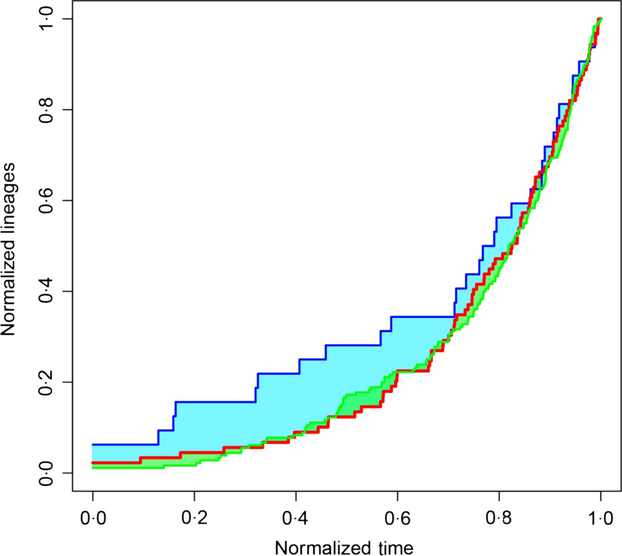
\includegraphics[scale=0.75]{nltt}
  \label{fig:nltt}
\end{figure}


% begin by sampling from the prior and setting all weights to equal

Next, we calculate the next tolerance $\varepsilon^*$. Before we explain how
this is done, we first need to define how we adjust the weights on the
particles. As explained above (see subsection~\ref{subsubsec:abcalg}), the idea
of sequential Monte-Carlo is to begin with the prior distribution $\pi$,
progress smoothly through a series of intermediate distributions $\pi_1,
\ldots, \pi_{n-1}$, and eventually arrive at the target posterior distribution
$\pi_n$. In the $k$th iteration, the distribution $\pi_k$ is approximated by
the particles and their weights. 

In contrast to most existing sequential Monte-Carlo methods, this
algorithm does not require the user to specify a sequence of decreasing
tolerances to approach the target posterior distribution. Rather, the
tolerances are computed adaptively at each step, starting from infinity at the
first iteration. 

The algorithm may be stopped when the tolerance reaches a
user-defined final value, or when the rate of acceptance of the
Metropolis-Hastings kernel reaches a user-defined threshold. Following a
heuristic applied by the authors~\autocite{del2012adaptive}, we used the latter
stopping criterion, accepting the SMC approximation to the posterior when the
\gls{MCMC} acceptance rate dropped below 1.5\%.

\subsection{Simulation experiments}

\subsubsection{Identification of separable parameters in kernel space}
\label{subsubsec:kernel}

Recall that our approximate Bayesian computation approach to fitting contact
network models involves simulating transmission trees under a wide variety of
parameter values, and then comparing these simulated trees to the true
transmission tree. Values which produce trees similar to the observed
transmission tree are distinguished as more likely than values which produce
trees very different from the truth. In order for this type of analysis to
succeed, it is critical that different parameter values produce different
looking trees. Otherwise, if many different values produce trees which are too
similar to each other, it will be impossible to distinguish which value is most
consistent with the real tree. Just as importantly, trees simulated with
similar parameter values must be similar to each other. In mathematical terms,
we require the trees simulated from distinct parameter values to be
\defn{separable} in tree space. The concept of separability is illustrated in
Figure~\ref{fig:separable}.

\begin{figure}[ht]
  \centering
  \includegraphics{separable}
  \caption[Separable versus non-separable pararameters in kernel space]{
    Separable versus non-separable parameters in kernel space. Trees have been
    simulated under three sets of parameters, represented as blue, red, and
    green. An observed tree is shown in black. Trees are layed out such that
    the distance between two trees corresponds to their similarity. In panel A,
    trees from the same parameter set are similar to each other, but different
    from other trees. The true tree is most consistent with the red parameters.
    In panels B and C, trees from the same parameter set are not similar to
    each other (B), or trees from different parameter sets are similar to each
    other (C). It's difficult to say which parameters the true tree is most
    consistent with.
  }
  \label{fig:separable}
\end{figure}

Before undertaking a complete ABC analysis, I analysed four simple contact
network models to determine whether their parameters could be separated in tree
kernel space. The four models are described in detail in
subsection~\ref{subsubsec:generative} of the introduction. Briefly, they are:
random networks, where each possible contact has a fixed probability of
occuring; preferential attachment networks, where highly connected nodes tend
to attract more contacts; small world networks, where nodes are connected to
their immediate neighbours and the occasional far-flung contact; and full
networks, where every possible connection is present. I will describe here only
the procedure and results for the preferential attachment networks. The details
of the other three types of graph can be found in the supplemental materials. A
graphical schematic of the analysis undertaken here is given in
Figure~\ref{fig:kernelexpt}.

\begin{figure}[ht]
  \centering
  \label{fig:kernelexpt}
  \includegraphics{kernel_expt}
  \caption[Schematic of first set of simulation experiments]{
    Schematic of first set of simulation experiments to determine separable
    parameters in kernel space, along with optimal tree kernel meta-parameters.
  }
\end{figure}

The method of testing for separability was described previously
in~\autocite{poon2015phylodynamic}, but I will reiterate it here for
completeness. As a concrete example, consider the attachment power parameter
\gls{alpha} of the preferential attachment networks. This parameter describes the
strength of attraction to highly connected nodes and is bounded below by zero
indicating no extra attraction. By qualitative observation, I determined that a
power of 2.0, which produced networks with very few ``hub'' nodes with
extremely high degree, was a suitable upper bound (see
Figure~\ref{fig:pabounds}). Therefore, I chose to test the values 0.5, 1.0, and
1.5 for separability. The other parameters were fixed: the number of nodes in
the network was 5000, and the mean degree of each node in the network was four.
As discussed in subsection~\ref{subsubsec:generative}, this is the smallest
mean degree value for preferential attachment networks which produces networks
which are more than trees. 

\begin{figure}[ht]
  \centering
  \label{fig:pabounds}
  \includegraphics{pa_power_bounds}
  \caption[Upper and lower bounds on preferential attachment power]{
    Qualitative justification for choice of zero and two as lower and upper
    bounds on preferential attachment power $\alpha$. (A) Preferential
    attachment network on 50 nodes with $\alpha = 0$, the lower bound enforced
    by the model. (B) Preferential attachment network on 50 nodes with $\alpha
    = 2$, where a few nodes have very high degree but the majority have very
    low degree. (C) Density plot of node degrees in a 5000-node network with
    $\alpha = 0$. The maximum degree of a node in this network was 24. (D)
    Density plot of node degrees in a 5000-node network with $\alpha = 2$. The
    maximum degree of a node in this network was 4942. 
  }
\end{figure}

For each of the values of $\alpha$, I generated 100 networks on 5000 nodes. An
epidemic was simulated over each network (see subsection X) until 1000 nodes
were infected, and 500 of those infected nodes were sampled to form a
transmission tree. This resulted in 300 total simulated transmission trees -
100 for each of the three values of $\alpha$. The data generation steps are
shown on the left side of Figure~\ref{fig:kernelexpt}. Next, I computed the
tree kernel~\autocite{poon2013mapping} (see
subsection~\ref{subsubsec:treeshape}) for each pair of trees. These values were
placed into a 300 $\times$ 300 kernel matrix, where the value at the $(i, j)$th
position was the tree kernel of the $i$th and $j$th trees. 

The tree kernel provides a pairwise similarity score between two trees. The
higher the kernel score, the more similar the trees are to each other.
Therefore, to have separability, we need trees simulated with the same value of
$\alpha$ to have high kernel scores with each other, but low kernel scores with
trees from different $\alpha$ values. We can visually check whether or not this
is true by laying out the trees as points on a graph, in such a way that trees
with high scores are close to each other, but trees with low scores are far
apart. This is accomplished by performing a kernel principal components
analysis (kPCA)~\autocite{scholkopf1998nonlinear} on the kernel matrix.
Briefly, ordinary principal components analysis (PCA) finds a lower dimensional
representation of points in a high dimensional space which preserves as much of
the variation in the data as possible. kPCA performs the same task, but using
the dot products of each pair of points as input, instead of the data points
themselves. A two-dimensional kPCA projection of the simulated trees is shown
in Figure~\ref{fig:pakpca}. The scenario just described - 500 samples from 1000
infected nodes - is the central panel. To ensure that the method could be used
in a variety of contexts, the same analysis was performed with 500 and 2000
infected nodes, as well as 100 and 1000 sampled tips. 

The next step was to quantify how well trees simulated with different $\alpha$
values could be distinguished from each other. As described
previously~\autocite{poon2015phylodynamic}, this was done by assessing the
accuracy of a support vector machine regression
(SVR)~\autocite{smola1997support}. Briefly, an SVR operates by finding a
hyperplane (in two dimensions, a line) such that the deviation of most of the
data points from the line is less than some prescribed threshold. Points
further away than this threshold are ignored in the model. I performed 1000
replicate 2-fold cross-validations of an SVR predicting preferential attachment
power on the simulated trees, using the \software{ksvm} function from
\software{kernlab}~\autocite{karatzoglou2004kernlab}. That is, the SVR was
trained on a random subset of 150 trees, and then used to predict $\alpha$ of
the remaining 150 trees. The predictions were correlated against the true
values of $\alpha$ to obtain an $R^2$, and this procedure was repeated 1000
times with different subsets of trees.

The cross-validation had the dual purpose of providing a means to selecting the
optimal meta-parameters to the tree kernel (see
subsection~\ref{subsubsec:treeshape}) - they are be those which provide the
highest average $R^2$. To this end, the cross-validation was repeated for
several values of $\lambda$ and $\sigma$ as shown in Figure~\ref{fig:kernelexpt}
Each combination was evaluated with and without multiplying the tree kernel by
the normalized lineages-through-time (nLTT) statistic, and was further repeated
for the scenarios with differing numbers of infected and sampled nodes
described above. To ensure that the tree kernel was the most appropriate
similarity measure to use for ABC, we also computed the $R^2$ of $\alpha$
against Sackin's index, a widely used tree balance statistic (see
subsection~\ref{subsubsec:treeshape}), by the same cross-validation procedure.

\subsubsection{Grid search}

The previous set of simulations were intended to investigate which contact
network parameters could and could not be inferred by examining transmission
trees. However, they tell us nothing about the accuracy or precision we might
expect when inferring those parameters numerically. As illustrated in
Figure~\ref{fig:accprec}, the ideal situation is one where we are accurate and
precise, and the worst situation is when we are precise but not accurate.

\begin{figure}[ht]
  \centering
  \includegraphics{acc_prec}
  \caption{Illustration of accurate vs. precise kernel score estimates}
  \label{fig:accprec}
\end{figure}

Figure~\ref{fig:gridsearch} shows a schematic of this experiment. A number of
representative values, here denoted $k$, were chosen for the parameter of
interest. In the case of preferential attachment power $\alpha$, I chose $k =
8$ testing values, namely $0, 0.25, \ldots, 2.0$. For each of these values, ten
networks on 5000 nodes were generated, an epidemic of 1000 nodes was simulated
over each, and a transmission tree of 500 tips was sampled. The resulting $10
\times k$ simulated transmission trees were referred to as the \defn{testing
trees}. In addition, I chose a further $n \gg k$ training values spanning the
range of the parameter. For $\alpha$, these were $0, 0.01, \ldots, 2.0$.
Fifteen trees were simulated in the same manner for each of these values,
referred to here as \defn{training trees}.

For each of the testing trees, I computed the tree kernel with all of the
training trees. This resulted in 15 kernel scores per training value. The
training value with the highest median kernel score was used as a point
estimate of the testing value. The kernel scores were then normalized to lie in
[0, 1], and an interval was found which contained 95\% of the area under the
curve and was of minimal width. This was used as a 95\% confidence interval for
the parameter.

\begin{figure}[ht]
  \centering
  \includegraphics{gridsearch_expt}
  \caption{Schematic of grid search simulation experiments.}
  \label{fig:gridsearch}
\end{figure}

\subsubsection{Approximate Bayesian computation}

Our final set of simulation experiments was to test the ABC-SMC algorithm on
simulated data. For each replicate, we generated a network on 5000 nodes,
simulated an epidemic over that network until 1000 nodes were infected, and
sampled either 500 or all 1000 of those nodes to form a transmission tree.
Priors were specified as follows: for the total number of nodes in the network,
$\Uniform(1000, 10000)$; for the number of infected nodes, $\Uniform(500,
2000)$; for the preferential attachment power, $\Uniform(0, 2)$. The mean
degree of nodes in the network was fixed at either 4, 10, or 16. The
algorithm was run with 1000 particles, and was stopped when the \gls{MCMC}
acceptance probability dropped below 1.5\%.

\subsection{Applications}

\subsubsection{HIV in British Columubia}


\section{Results}
\subsection{Analysis of \acrlong{BA} model}



\subsubsection*{Classifiers for BA model parameters based on tree shape}



Trees simulated under different values of \gls{alpha} were visibly quite
distinct (\cref{fig:alphatrees}). In particular, higher values of \gls{alpha}
produce networks with a small number of highly connected nodes which, once
infected, are likely to transmit to many other nodes. This results in a more
unbalanced, ladder-like structure in the phylogeny, compared to networks with
lower \gls{alpha} values. None of the other three parameters produced trees
which were as easily distinguished from each other
(\cref{fig:Itrees,fig:mtrees,fig:Ntrees,fig:Itrees}).  Sackin's index, which
measures tree imbalance, was significantly correlated with all four parameters
    (for $\alpha$, $I$, $m$, and $N$ respectively: Spearman's rho =
     0.85,
     \ensuremath{-0.12},
     \ensuremath{-0.13},
     0.09;
     $p$-values
     ${<}10^{-5}$,
     $0.003$,
     ${<}10^{-5}$,
     ${<}10^{-5}$).
The ratio of internal to terminal branch lengths was negatively correlated with
\gls{alpha} and \gls{I}, and positively correlated with \gls{m} and \gls{N}
  (Spearman's rho
    \ensuremath{-0.84},
    \ensuremath{-0.69},
    0.1,
    0.18;
  all $p < 10^{-5}$).

\begin{figure}[ht]
  \centering
  \includegraphics[width=\textwidth]{kernel-alpha-tree.pdf}
  \caption[Simulated transmission trees under three different values of BA parameter $\alpha$]{
    Simulated transmission trees under three different values of BA parameter
    $\alpha$. Epidemics were simulated on \gls{BA} networks of 5000 nodes, with
    \gls{alpha} equal to 0.5, 1.0, or 1.5, until 1000 individuals were
    infected. Transmission trees were created by sampling 500 infected nodes.
    Higher \gls{alpha} values produced networks with a small number of
    highly-connected nodes, resulting in highly unbalanced, ladder-like trees.
  }
  \label{fig:alphatrees}
\end{figure}

\Cref{fig:kpca} shows \gls{kPCA} projections of the simulated trees onto the
first two principal components of the kernel matrix. The figure shows only the
simulations with 500-tip trees and 1000 infected nodes. The three \gls{alpha}
and \gls{I} values considered are well separated from each other in feature
space. On the other hand, the three \gls{N} values overlap significantly, and
the three \gls{m} values are virtually indistinguishable. Similar observations
can be made for other values of \gls{I} and the number of tips
(\cref{fig:alphakpca,fig:Nkpca,fig:Ikpca,fig:mkpca}). The values of \gls{I} and
\gls{N} separated more clearly with larger numbers of tips, and in the case of
\gls{N}, larger epidemic sizes.

\begin{figure}[ht]
  \centering
  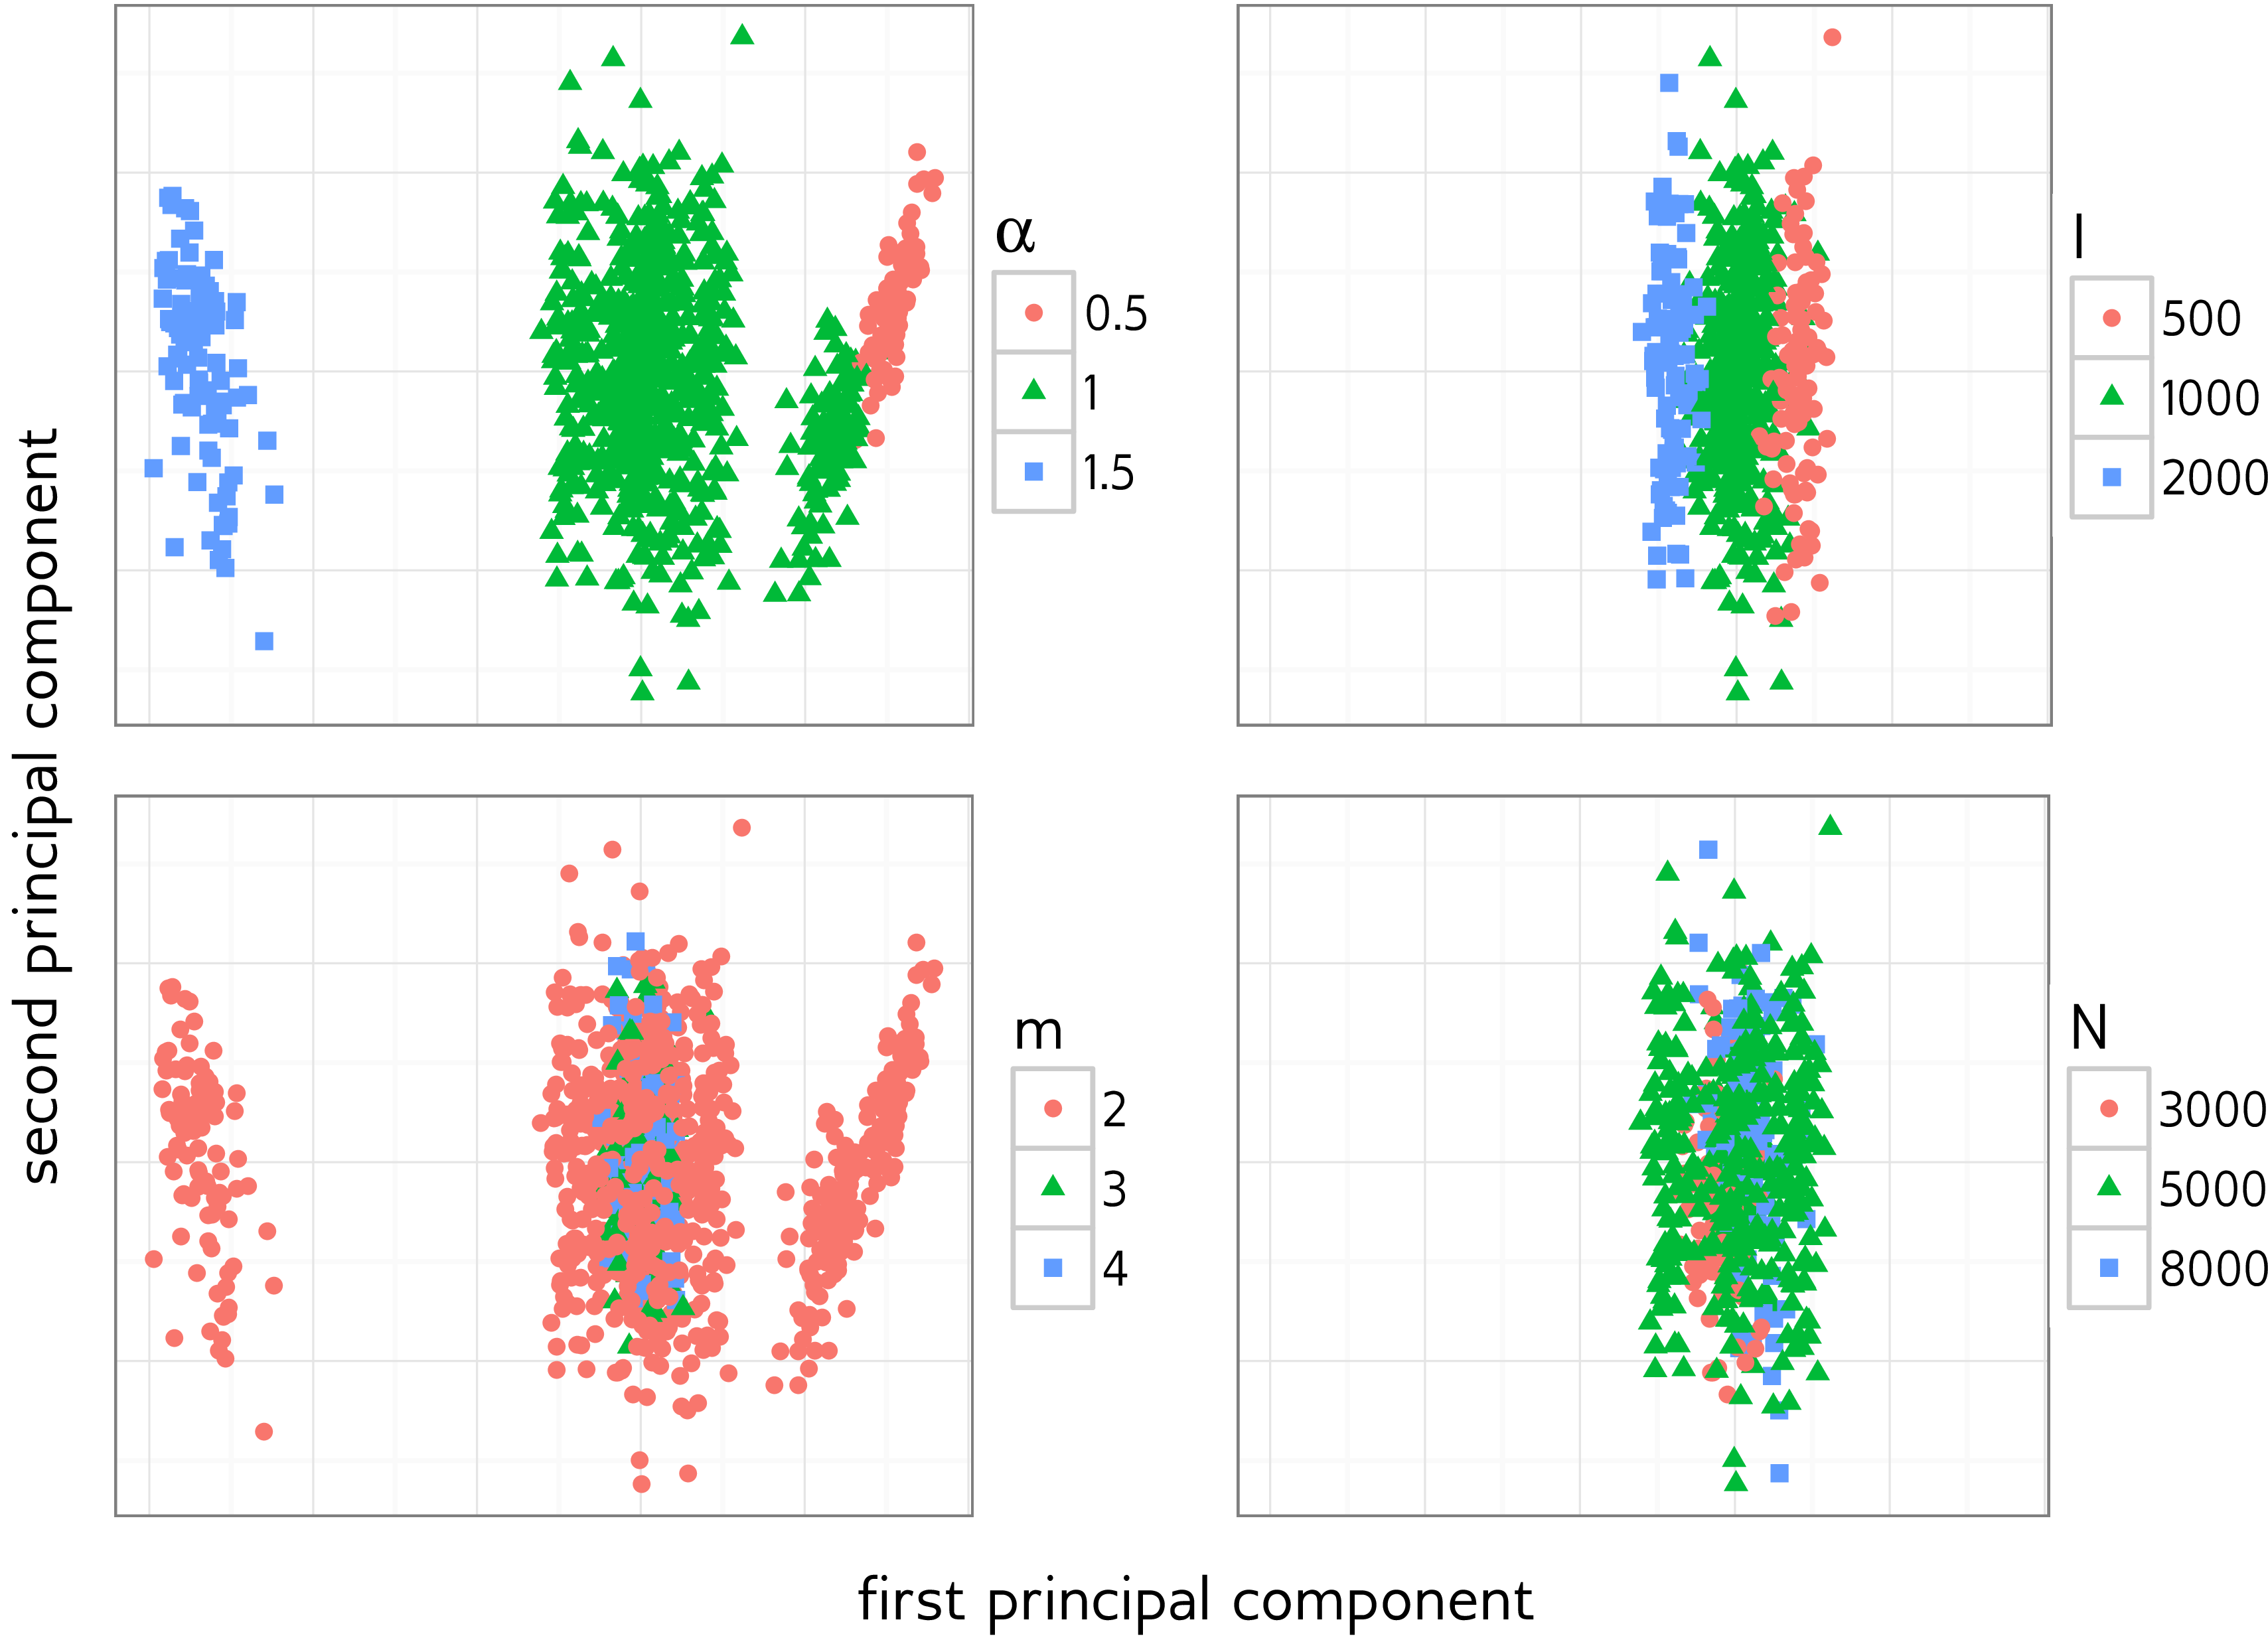
\includegraphics{kernel-kpca.pdf}
  \caption[Kernel-PCA projections of simulated trees under varying BA
           parameter values.]{
    Each parameter of the \gls{BA} model was individually varied to produce 300
    simulated trees. Kernel matrices were formed from all pairwise kernel
    scores among each set of 300 trees. The trees were projected onto the first
    two principal components of the kernel matrix calculated using \gls{kPCA}.
    All trees had 500 tips. The parameters not being varied were set to
    \gls{alpha} = 1, \gls{I} = 1000, \gls{m} = 2, and \gls{N} = 5000. The tree
    kernel meta-parameters were $\lambda = 0.3$ and $\sigma = 4$.
  }
  \label{fig:kpca}
\end{figure}



Accuracy of the \gls{kSVR} classifiers varied based on the parameter being
tested (\cref{fig:rsquared}, left). Classifiers based on two other tree
statistics, the \gls{nltt} and Sackin's index, generally exhibited worse
performance than the tree kernel, although the magnitude of the disparity
varied between the parameters (\cref{fig:rsquared}, centre and right). The
results were largely robust to variations in the tree kernel meta-parameters
$\lambda$ and $\sigma$, although accuracy varied between different epidemic and
sampling scenarios
(\cref{fig:alphacrossv,fig:mcrossv,fig:Icrossv,fig:Ncrossv}).

When classifying $\alpha$, the \gls{kSVR} classifier had an average $R^2$ of 
    0.92,
compared to 
    0.56
for the \gls{nltt}-based SVR, and
    0.75
for the linear regression against Sackin's index. There was little variation
about the mean for different tree and epidemic sizes. No classifier could
accurately identify the $m$ parameter in any epidemic scenario, with average
$R^2$ values of 
  0.12 for \gls{kSVR},
  0.01 for the \gls{nltt}, and
  0.06
for Sackin's index. Again, there was little variation in accuracy between
epidemic scenarios, although the accuracy of the \gls{kSVR} was slightly higher
on 1000-tip trees 
    (average $R^2$ 
     0.01,
     0.11,
     0.32
     for 100, 500, and 1000 tips respectively).

The accuracy of classifiers $I$ varied significantly with the number of tips in
the tree. For 100-tip trees, the average $R^2$ values were
  0.7,
  0.55, and
  0.02
for the tree kernel, \gls{nltt}, and Sackin's index respectively. For 500-tip
trees, the values increased to
  0.93,
  0.83, and
  0.07.
Finally, the performance of classifiers for $N$ depended heavily on the
epidemic scenario. The $R^2$ of the \gls{kSVR} classifier ranged from
  0.08
for the smallest epidemic and smallest sample size, to
  0.82
for the largest. Likewise, $R^2$ for the \gls{nltt}-based SVR ranged from 
  0.01
to
  0.54.
Sackin's index did not accurately classify $N$ in any scenario, with an average
$R^2$ of
  0.03
and little variation between scenarios.

\begin{figure}[ht]
  \centering
  \includegraphics[width=\textwidth]{kernel-rsquared.pdf}
  \caption[Cross-validation accuracy of kernel-SVR, nLTT-based SVR, and
  Sackin's index regression classifiers for BA model parameters.]{
      Cross-validation accuracy of kernel-SVR classifier (left), SVR classifier
      using \gls{nltt} (centre), and linear regression using Sackin's index
      (right) for \gls{BA} model parameters. Kernel meta-parameters were set to
      $\lambda = 0.3$ and $\sigma = 4$. Each point was calculated based on 300
      simulated transmission trees over networks with three different values of
      the parameter being tested. Vertical lines are empirical 95\% confidence
      intervals based on 1000 two-fold cross-validations.
  }
  \label{fig:rsquared}
\end{figure}

\subsubsection*{Marginal parameter estimates with grid search}



The accuracy of grid search estimates largely paralleled that of the \gls{kSVR}
classifiers. \Cref{fig:gridest} shows point estimates and 95\% highest density
intervals for each of the \gls{BA} parameters, for one replicate experiment
with 500-tip trees. Plots showing the point estimates for all replicates can be
found in \cref{fig:gridptalpha,fig:gridptI,fig:gridptm,fig:gridptN}. For all
parameters except $m$, the error of point estimates was negatively correlated
with the number of sampled tips in the tree (for
\gls{alpha}, \gls{I}, and \gls{N} respectively: Spearman's $\rho$ = 
    \ensuremath{-0.22},
    \ensuremath{-0.51},
    \ensuremath{-0.16};
$p$-values
    $4\!\times\!10^{-4}$,
    ${<}10^{-5}$,
    $0.01$).
The highest density intervals obtained for all parameters were extremely wide,
occupying $>$75\% of the grid in all cases (\cref{fig:gridest}).

The \gls{alpha} parameter was the most accurately estimated, with point
estimates having an average deviation of 
    0.14
from the true value, on a grid from 0 to 2. The error of point estimates varied
significantly between true values of \gls{alpha}
    (one-way \gls{ANOVA}, $p$ ${<}10^{-5}$). In
particular, errors were lower for the values \gls{alpha} = 1.0 and 1.25 than
for the other values
    (average errors 
    0.03
    for \gls{alpha} = 1.0 or 1.5 vs.
    0.17
    for \gls{alpha} $\neq$ 1.0 or 1.5),
and this difference was significant
    (Wilcoxon rank-sum test, $p {<}10^{-5}$,
     \cref{fig:gridptalpha}).
These two values exhibited different qualitative behaviour than the other
values in terms of the distribution of kernel scores along the grid
(\cref{fig:gridalpha}). In particular, there was a pronounced peak in scores
around the true value, in contrast to the other values where the scores were
flat around the true value. The effect was most obvious for the value
\gls{alpha} = 1.25.

The average absolute error of the point estimates for \gls{I} was 
    310 individuals,
on a grid of 500 to 5000, and these errors differed between true values of
\gls{I}
    (one-way \gls{ANOVA}, $p =0.001$).
The errors for $2000 \leq I \leq 3000$ were higher than those for the other
values
    (average errors
     430
     for $2000 \leq I \leq 3000$ vs.
     250
     for $I < 2000$ or $I > 3000$),
and this difference was significant
    (Wilcoxon rank-sum test, $p =6\!\times\!10^{-4}$,
     \cref{fig:gridptI}).
Kernel score distributions for all test values exhibited a similar rounded
shape (\cref{fig:gridI}). 

The average error for \gls{m} was
    1.31 edges per vertex,
on a grid from 1 to 6. The error varied significantly between the true values
of \gls{m} 
    (one-way \gls{ANOVA}, $p {<}10^{-5}$).
Errors for the value \gls{m} = 1 were lower than the other values
    (average errors
    0.1
    for $m = 1$ vs.
    1.55
    for $m > 1$),
and this difference was significant
    (Wilcoxon rank-sum test, $p {<}10^{-5}$,
     \cref{fig:gridptm}).
The value $m = 1$ causes the network to take on a distinct shape relative to
higher \gls{m} values, namely a tree (\ie there are no cycles, see
\cref{subsec:treeshape}). The kernel score distribution had a peak at $m = 1$
when this was the true value, and a valley at $m = 1$ when the true value of
$m$ was greater that 1 (\cref{fig:gridm}).

The average error for \gls{N} was 
    2419 individuals,
on a grid from 1000 to 15000, and was varied significantly with the true value
of \gls{N}
    (one-way \gls{ANOVA}, $p {<}10^{-5}$).
The errors were lower for $N \leq 3000$
    (average errors
     740
     for $N \leq 3000$ vs.
     2979
     for $N > 3000$),
and this difference was significant
    (Wilcoxon rank-sum test, $p {<}10^{-5}$,
     \cref{fig:gridptN}).
The kernel score distribution had a peak at $N = 1000$ when this was the true
value, and a valley there otherwise (\cref{fig:gridN}). Except for this valley,
the distributions were flat for $N > 3000$.

\begin{figure}[ht]
  \centering
  \includegraphics[width=\textwidth]{gridsearch-example}
  \caption[Grid search estimates of \gls{BA} model parameters.]{Point estimates
      and 95\% highest density intervals for each \gls{BA} model parameter,
      obtained using grid search. Networks and transmission trees were
      simulated over a grid of values for each parameter while holding the
      others fixed. For a subset of the grid values ($x$-axis), test networks
      and trees were created and compared to each tree on the grid using the
      tree kernel. The kernel scores along the grid were normalized to resemble
      a probability distribution, from which the mode and highest density
      interval were calculated. Shown values correspond to one replicate
      experiment, with trees of size 500.
  } 
  \label{fig:gridest}
\end{figure}

\subsubsection*{Joint parameter estimates with kernel-assisted ABC}



\Cref{fig:abcptm2} shows \gls{MAP} point estimates of the BA model parameters
obtained with kernel-assisted ABC on simulated data. The estimates shown correspond only
to the simulations where the $m$ parameter was set to 2, however the results
for $m = 3$ and $m = 4$ were similar (\cref{fig:abcptm3,fig:abcptm4}). Average
boundaries of 95\% HPD intervals are given in \cref{tab:abchpd}.

The accuracy of the parameter estimates obtained with kernel-assisted ABC
paralleled the results from the \gls{kSVR} classifier. Of the four parameters,
$\alpha$ was the most accurately estimated, with point estimates having a
median [IQR] absolute error of 
    0.08 
    [0.05 - 
    0.17].
The errors when the true value of $\alpha$ was zero were significantly greater
than those for the other values 
    (Wilcoxon rank-sum test, $p$ = $0.0078$).
Errors in estimating $\alpha$ also varied with the true value of $m$ just at
the threshold of statistical significance
    (one-way ANOVA, $p 
    =0.05$),
but did not vary across the true value of $I$ (one-way ANOVA). Estimates for
$I$ were relatively accurate, with point estimate errors of
    395 
    [207 - 
    683] individuals.
These errors were significantly higher when the true value of $\alpha$ was
at least 1
    (Wilcoxon rank-sum test, $p$ = $0.0077$)
and when the true value of $I$ was 2000 ($p < 10^{-5}$). The true value of $m$
did not affect the estimates of $I$ (one-way ANOVA).

The $m$ parameter was estimated correctly in only
    27 \%
of simulations, barely better than random guessing. The true values of the
other parameters did not significantly affect the estimates of $m$ (both
one-way ANOVA). Finally, the total number of nodes $N$ was consistently
over-estimated by about a factor of two
    (error 5987 
    [2060 - 
     7999] individuals).
No parameters influenced the accuracy of the $N$ estimates (all one-way ANOVA).

\begin{figure}[ht]
  \centering
  \includegraphics[width=\textwidth]{abc-point-estimate-m2}
  \vspace{6pt}
  \caption[
    \Acrlong{MAP} point estimates for \gls{BA} model parameters obtained by
    running \software{netabc} on simulated data, for simulations with \gls{m} =
    2.
  ]{
    \Acrlong{MAP} point estimates for \gls{BA} model parameters obtained by
    running \software{netabc} on simulated data, for simulations with \gls{m} =
    2. Dashed lines indicate true values. (A) Estimates of \gls{alpha} and
    \gls{I} which were varied in these simulations against known values. (B)
    Estimates of \gls{m} and \gls{N} which were held fixed in these simulations
    at the values \gls{m} = 2 and \gls{N} = 5000.
  }
  \label{fig:abcptm2}
\end{figure}

\begin{table*}[ht]
  \centering
  % latex table generated in R 3.2.3 by xtable 1.8-2 package
% Fri Jun 17 12:51:45 2016
\begin{tabular}{lr>{\raggedleft\arraybackslash}p{2.5cm}>{\raggedleft\arraybackslash}p{2.5cm}>{\raggedleft\arraybackslash}p{2.5cm}}
  \hline
Parameter & True value & Mean point estimate & Mean HPD lower bound & Mean HPD upper bound \\ 
  \hline
$\alpha$ & 0.0 & 0.36 & 0.01 & 0.81 \\ 
   & 0.5 & 0.43 & 0.04 & 0.83 \\ 
   & 1.0 & 0.90 & 0.51 & 1.09 \\ 
   & 1.5 & 1.52 & 1.26 & 1.81 \\ 
  $I$ & 1000 & 1450 & 651 & 2592 \\ 
   & 2000 & 2622 & 1114 & 4080 \\ 
  $m$ & 2 & 2.96 & 2.00 & 5.00 \\ 
   & 3 & 3.04 & 2.04 & 4.96 \\ 
   & 4 & 3.17 & 1.88 & 5.00 \\ 
  $N$ & 5000 & 9041 & 2613 & 14659 \\ 
   \hline
\end{tabular}

  \caption[
      Average maximum \textit{a posteriori} point estimates and 95\% highest
      posterior density (HPD) interval widths for BA model parameter estimates
      obtained with kernel-assisted ABC.
  ]{
      Average maximum \textit{a posteriori} point estimates and 95\% highest
      posterior density (HPD) interval widths for BA model parameter estimates
      obtained with kernel-assisted ABC. Three transmission trees were simulated under
      each combination of the listed parameter values, and the parameters were
      estimated with kernel-assisted ABC without training.
  }
  \label{tab:abchpd}
\end{table*}



The dispersion of the ABC approximation to the posterior also varied between
the parameters, with narrower HPD intervals for the parameters with more
accurate point estimates (\cref{tab:abchpd}). \Cref{fig:abcex} shows
the distributions for for one simulation. Equivalent plots for one replicate
simulation with each studied parameter combination can be found in
\cref{fig:0.0-1000-2-5000-0,fig:0.5-1000-2-5000-0,fig:1.0-1000-2-5000-0,fig:1.5-1000-2-5000-0,fig:0.0-2000-2-5000-0,fig:0.5-2000-2-5000-0,fig:1.0-2000-2-5000-0,fig:1.5-2000-2-5000-0,fig:0.0-1000-3-5000-0,fig:0.5-1000-3-5000-0,fig:1.0-1000-3-5000-0,fig:1.5-1000-3-5000-0,fig:0.0-2000-3-5000-0,fig:0.5-2000-3-5000-0,fig:1.0-2000-3-5000-0,fig:1.5-2000-3-5000-0,fig:0.0-1000-4-5000-0,fig:0.5-1000-4-5000-0,fig:1.0-1000-4-5000-0,fig:1.5-1000-4-5000-0,fig:0.0-2000-4-5000-0,fig:0.5-2000-4-5000-0,fig:1.0-2000-4-5000-0,fig:1.5-2000-4-5000-0}. HPD intervals around $\alpha$ and $I$ were often narrow
relative to the region of nonzero prior density, whereas the intervals for $m$
and $N$ were more widely dispersed.

\begin{figure}[ht]
    \centering
    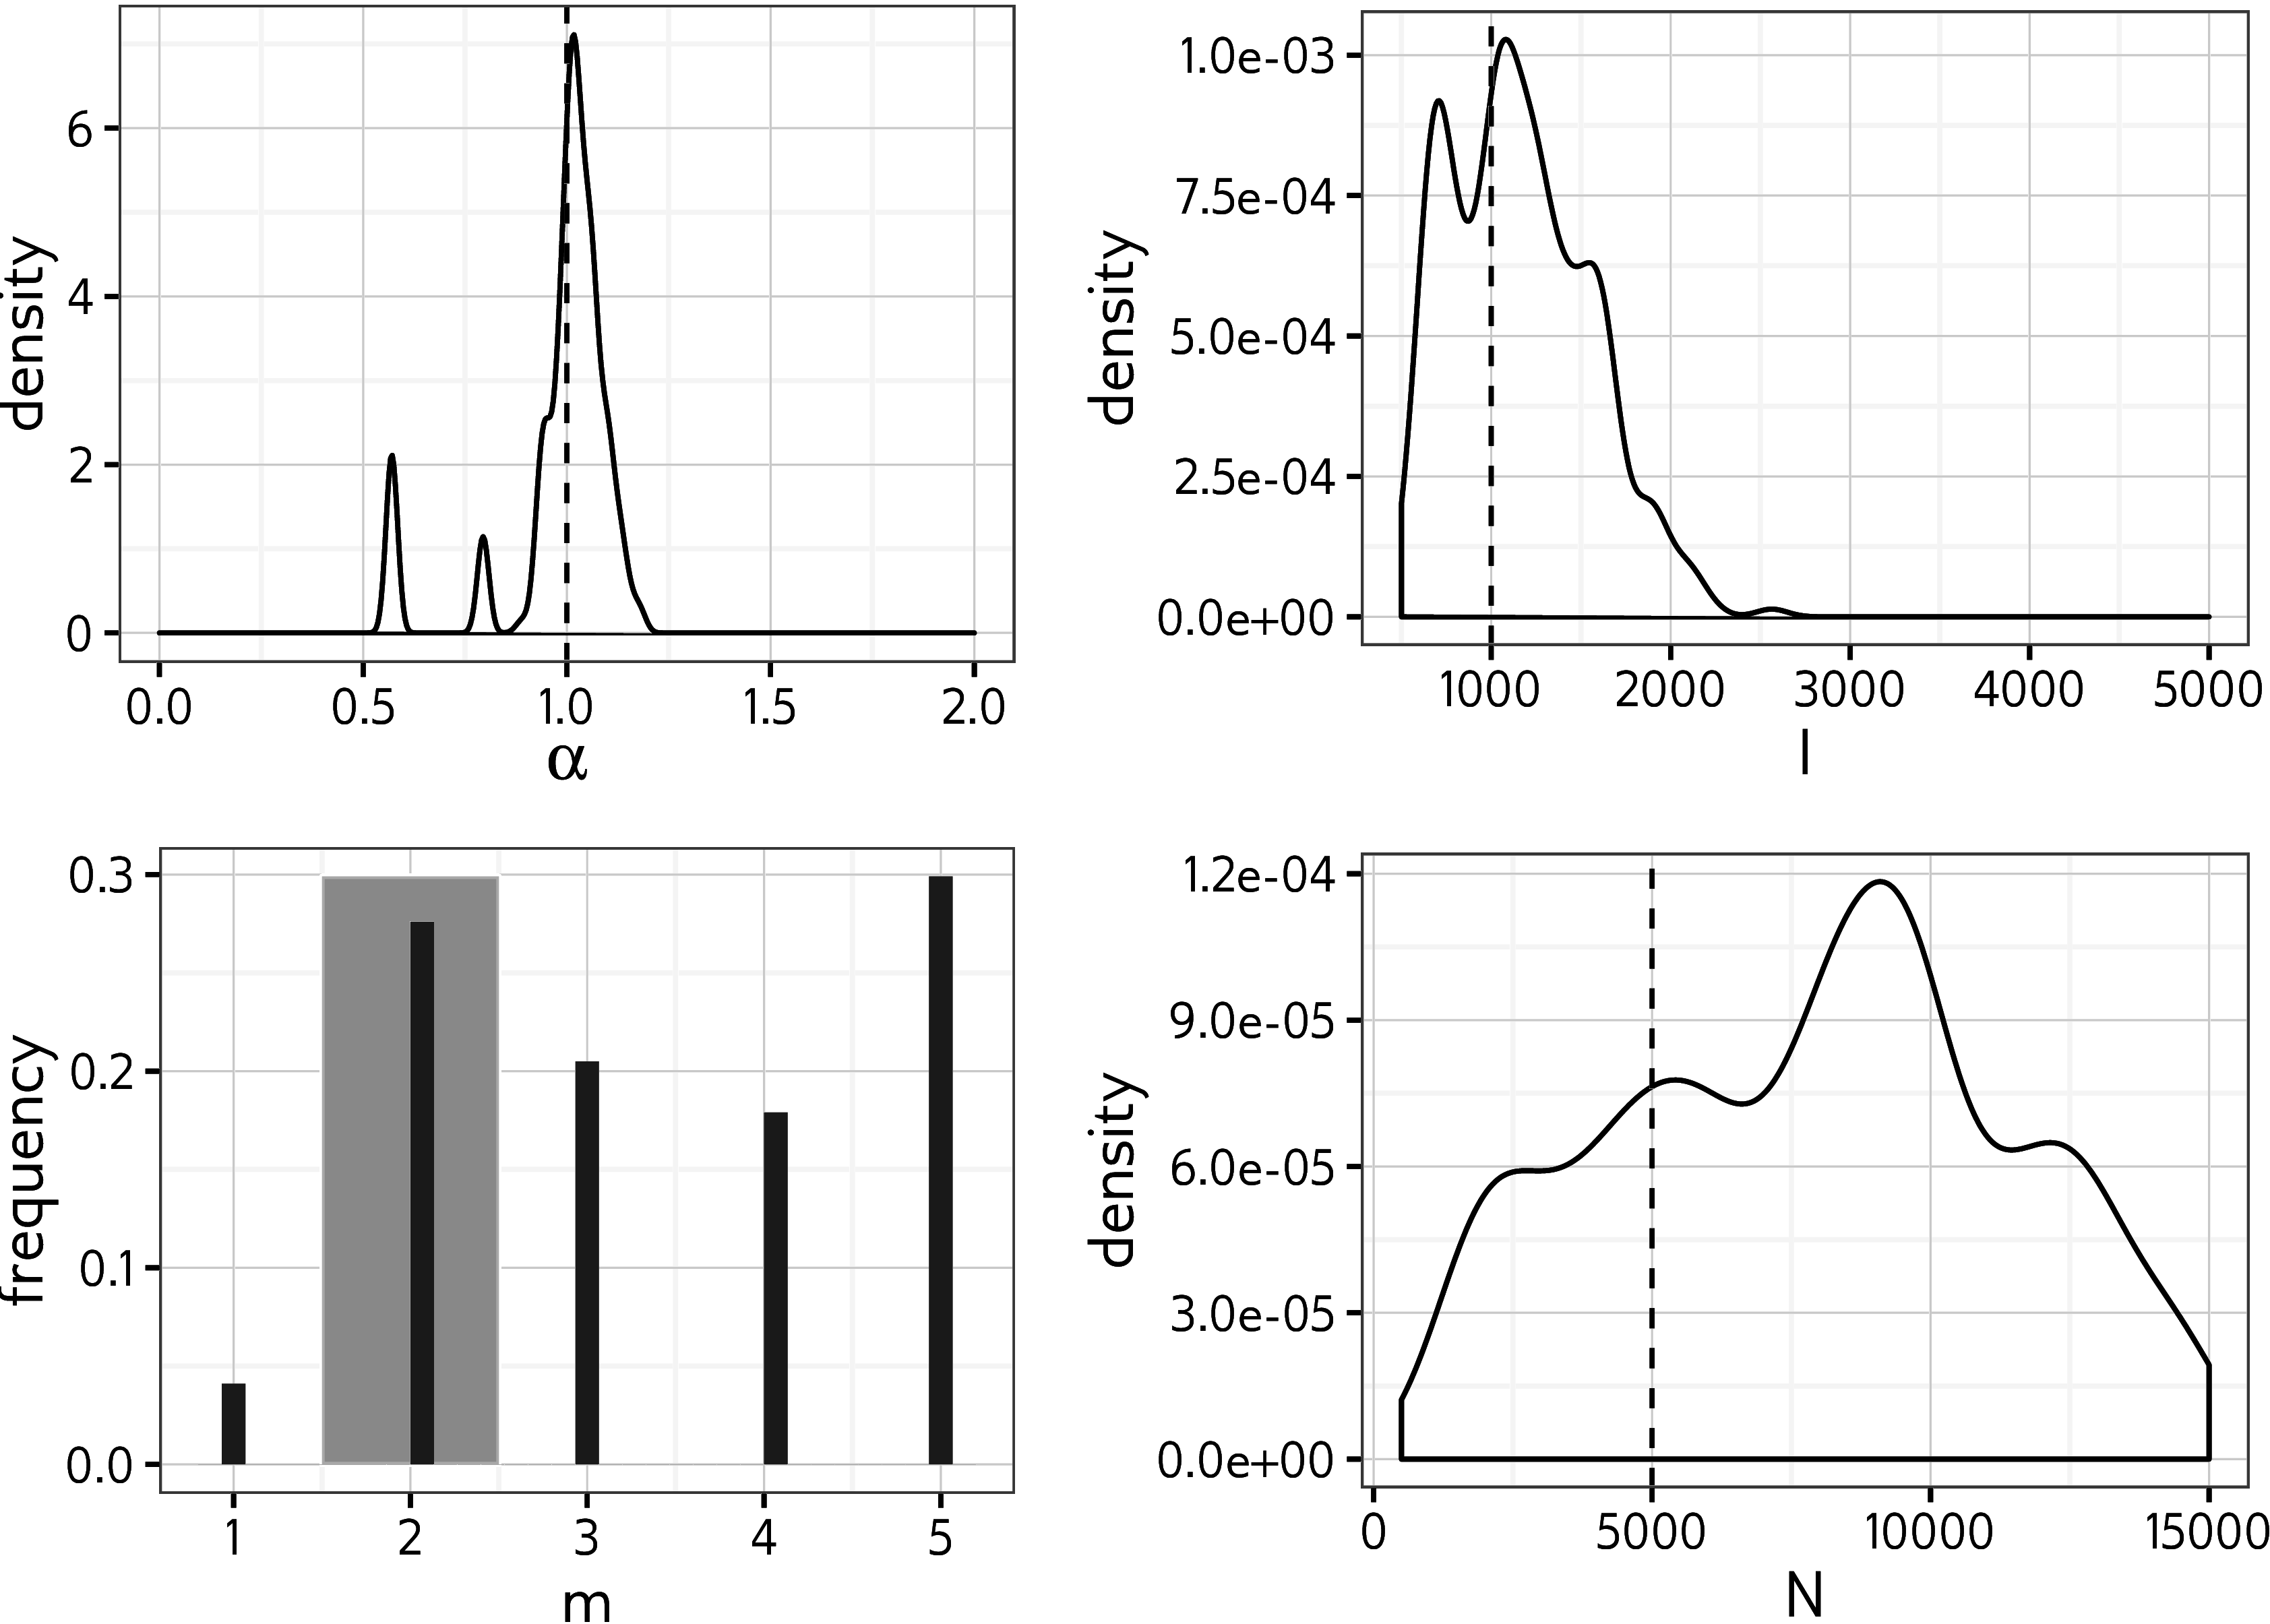
\includegraphics[width=\textwidth]{abc-posterior-example}
  \vspace{6pt}
  \caption{
    Marginal posterior distributions of BA model parameters estimated
    with kernel-assisted ABC for a single simulated transmission tree. Dotted
    lines and shaded polygon indicate true values.
  }
  \label{fig:abcex}
\end{figure}



To test the effect of model misspecification, we simulated one network where
the nodes exhibited heterogeneous preferential attachment power (half 0.5, the
other half 1.5), with $m$ = 2, $N$ = 5000, and $I$ = 1000. The MAP [95\%
HPD] estimates for each parameter were: 
$\alpha$, 
  1.1 
  [0.6 -
   1.16];
$I$,
  1119 
  [662 -
   4455];
$m$,
  3 
  [1 -
   5];
$N$,
  12678 
  [3367-
   14977].
The approximate posterior distributions for this simulation are shown in
\cref{fig:mixed}. To test the effect of sampling bias, we sampled one
transmission tree in a peer-driven fashion, where the probability to sample a
node was twice as high if one of its peers had already been sampled. The
parameters for this experiment were $N$ = 5000, $m$ = 2, $\alpha$ = 0.5, and
$I$ = 2000. The estimated values were
$\alpha$, 
  0.23 
  [0.01 -
   0.63];
$I$,
  2398 
  [1419 -
   3767];
$m$,
  3 
  [2 -
   5];
$N$,
  9761 
  [2836 -
   14788].
The approximate posterior distributions are shown in \cref{fig:peerdriven}. Both
of these results were in line with estimates obtained on other simulated
datasets (\cref{tab:abchpd}), although the estimate of peer-driven sampling for
$\alpha$ was somewhat lower than typical.

%<<abc_glm, include=FALSE>>=
%    source("global.R")
%    options(scipen=-1, digits=2)
%@
%
%<<alpha_glm, include=FALSE>>=
%    # alpha_error is influenced by alpha and m but not I
%    stopifnot(alpha.glm[Parameter == "alpha", min(p) < 0.05])
%    stopifnot(alpha.glm[Parameter == "m", min(p) < 0.05])
%    stopifnot(alpha.glm[Parameter == "I", min(p) > 0.05])
%
%    # alpha_error is correlated with true_alpha
%    alpha.test <- d[,cor.test(alpha_error, true_alpha, method="spearman")]
%    stopifnot(alpha.test$p.value < 0.05)
%
%    # alpha_error is not correlated with true_m
%    alpha.m.cor <- d[,cor.test(alpha_error, true_m)]
%    stopifnot(alpha.m.cor$p.value < 0.05)
%@
%
%We used \software{netabc} to estimate the parameters of the \gls{BA} model on
%simulated trees where the true parameter values were known. Point estimates for
%each parameter are shown in \cref{fig:abcptm2} for the simulations with \gls{m} =
%2. The results for the other values of \gls{m} were similar
%(\cref{fig:abcptm3,fig:abcptm4}). The median [IQR] absolute error of estimates
%of \gls{alpha} across all simulations was
%    d[,median(alpha_error)] 
%    [d[,quantile(alpha_error, 0.25)]-d[,quantile(alpha_error, 0.75)]].
%\Gls{GLM} analysis indicated that the true values of both \gls{alpha} and
%\gls{m} had significant effects on the error in estimated \gls{alpha}
%    ($p$ values $pp(alpha.glm[Parameter == "alpha", min(p)], eq=FALSE)$
%     $pp(alpha.glm[Parameter == "m", min(p)], eq=FALSE)$,
%     \cref{tab:glmalpha}),
%but the true value of \gls{I} did not. There was a significant negative
%correlation between the true value of \gls{alpha} and the error
%    (Spearman's $\rho$ = round(alpha.test$estimate, 2),
%     $p pp(alpha.test$p.value, eq=TRUE)$).
%There was a negative correlation between \gls{m} and the error in \gls{alpha}
%    (Spearman's $\rho$ = round(alpha.m.cor$estimate, 2),
%    $p pp(alpha.m.cor$p.value, eq=FALSE)$).
%
%<<I_glm, include=FALSE>>=
%    # I_error is influenced by alpha and I but not by m
%    stopifnot(I.glm[Parameter == "alpha", min(p) < 0.05])
%    stopifnot(I.glm[Parameter == "m", min(p) > 0.05])
%    stopifnot(I.glm[Parameter == "I", min(p) < 0.05])
%
%    # correlation between I_error and true_alpha
%    I.alpha.cor <- d[,cor.test(I_error, true_alpha, method="spearman")]
%    stopifnot(I.alpha.cor$p.value < 0.05)
%
%    # correlation between I_error and true_I
%    I.I.cor <- d[,cor.test(I_error, true_I, method="spearman")]
%    stopifnot(I.alpha.cor$p.value < 0.05)
%@
%
%The mean error in the estimated value of \gls{I} was
%    d[,round(median(I_error))] 
%    [d[,round(quantile(I_error, 0.25))]-d[,round(quantile(I_error, 0.75))]],
%an over-estimate of roughly a factor of 1.5
%(\cref{fig:abcptm2,fig:abcptm1,fig:abcptm3,fig:abcptm4}). \Gls{GLM} analysis
%indicated a relationship between the error in estimated \gls{I}, and the true
%values of \gls{alpha} and \gls{I}
%    ($p$ values $pp(I.glm[Parameter == "alpha", min(p)], eq=FALSE)$
%     $pp(alpha.glm[Parameter == "I", min(p)], eq=FALSE)$,
%     \cref{tab:glmalpha}),
%but not the true value of \gls{m}. There was a significant correlation between 
%the true value of \gls{alpha} and the error in estimated \gls{I}
%    (Spearman's $\rho$ = I.alpha.cor$estimate,
%     $p pp(I.alpha.cor$p.value, eq=TRUE)$),
%and between the true value of \gls{I} and the error in estimated \gls{I}
%    (Spearman's $\rho$ = I.I.cor$estimate,
%     $p pp(I.I.cor$p.value, eq=TRUE)$).
%
%<<m_glm, include=FALSE>>=
%    # effects of parameters on m_error
%    stopifnot(m.glm[Parameter == "m", min(p)] < 0.05)
%    stopifnot(m.glm[Parameter == "alpha", min(p)] > 0.05)
%    stopifnot(m.glm[Parameter == "I", min(p)] > 0.05)
%
%    # m was only estimated correctly in just over 20\% of simulations with m > 2
%    m.tbl <- prop.table(table(d[true_m > 1,m_error]))
%    stopifnot(m.tbl[1] > 0.2 & m.tbl[1] < 0.3)
%
%    # with m = 1, over 95% of simulations are right
%    m1.est <- d[true_m == 1, m_error]
%    stopifnot(sum(m1.est == 0) / length(m1.est) > 0.95)
%    stopifnot(sum(m1.est == 0) / length(m1.est) < 1)
%@
%
%\gls{GLM} analysis showed an effect of the true value of \gls{m} on the error
%in the estimated \gls{m}
%    ($p pp(m.glm[Parameter == "m", min(p)])$,
%     \cref{tab:glmm}).
%When the true value of \gls{m} was 1, the correct value was recovered by
%\software{netabc} in virtually every case
%    (sum(m1.est == 0) out of length(m1.est) simulations).
%However, when the true value of \gls{m} was 2 or higher, the correct value was
%recovered in only 
%    as.integer(m.tbl[1] * 100)\%
%of simulations, little better than random guessing. The \gls{GLM} analysis did
%not indicate any effects of the true parameter values on the error in estimated
%\gls{m} (\cref{tab:glmm}).
%
%<<N_glm, include=FALSE>>=
%    # alpha_error is influenced by alpha and m but not I
%    stopifnot(N.glm[Parameter == "alpha", min(p) < 0.05])
%    stopifnot(N.glm[Parameter == "I", min(p) < 0.05])
%    stopifnot(N.glm[Parameter == "m", min(p) > 0.05])
%
%    N.alpha.test <- d[,wilcox.test(.SD[true_alpha == 1.5, N_error], 
%                                   .SD[true_alpha < 1.5, N_error])]
%    stopifnot(N.alpha.test$p.value < 0.05)
%    N.I.test <- d[,wilcox.test(.SD[true_I == 3000, N_error], 
%                               .SD[true_I < 3000, N_error])]
%    stopifnot(N.I.test$p.value < 0.05)
%@
%
%Finally, the total number of nodes \gls{N} was consistently over-estimated by
%about a factor of two
%    (error d[,format(median(N_error), scientific=FALSE)] 
%    [d[,format(quantile(N_error, 0.25), scientific=FALSE)] - 
%     d[,format(quantile(N_error, 0.75), scientific=FALSE)]]).
%The fitted \gls{GLM} indicated that the true values of both \gls{alpha} and
%\gls{I} had an effect on the error in the estimated \gls{N}
%    ($p$-values $pp(N.glm[Parameter == "alpha", min(p)], eq=FALSE)$ and 
%     $pp(N.glm[Parameter == "I", min(p)], eq=FALSE)$,
%     \cref{tab:glmN}),
%but that the true value of \gls{m} did not. The error in the estimated \gls{N}
%when \gls{alpha} was equal to 1.5 was slightly lower than for other values of
%\gls{alpha}
%    (median [IQR] error rates 
%     d[true_alpha == 1.5, format(median(N_error), scientific=FALSE)] 
%    [d[true_alpha == 1.5, format(quantile(N_error, 0.25), scientific=FALSE)] - 
%     d[true_alpha == 1.5, format(quantile(N_error, 0.75), scientific=FALSE)]]
%     for \gls{alpha} = 1.5 vs. 
%     d[true_alpha < 1.5, format(median(N_error), scientific=FALSE)] 
%    [d[true_alpha < 1.5, format(quantile(N_error, 0.25), scientific=FALSE)] - 
%     d[true_alpha < 1.5, format(quantile(N_error, 0.75), scientific=FALSE)]]
%     for \gls{alpha} < 1.5),
%and this difference was statistically significant
%    (Wilcoxon rank-sum test, $p pp(N.alpha.test$p.value, eq=TRUE)$).
%Similarly, the error in the estimated \gls{N} when \gls{I} was equal to 3000 was
%lower than for other values of \gls{I}
%    (median [IQR] error rates 
%     d[true_I == 3000, format(median(N_error), scientific=FALSE)] 
%    [d[true_I == 3000, format(quantile(N_error, 0.25), scientific=FALSE)] - 
%     d[true_I == 3000, format(quantile(N_error, 0.75), scientific=FALSE)]]
%     for \gls{I} = 3000 vs. 
%     d[true_alpha < 3000, format(median(N_error), scientific=FALSE)] 
%    [d[true_alpha < 3000, format(quantile(N_error, 0.25), scientific=FALSE)] - 
%     d[true_alpha < 3000, format(quantile(N_error, 0.75), scientific=FALSE)]]
%     for \gls{I} < 3000),
%and this difference was statistically significant
%    (Wilcoxon rank-sum test, $p pp(N.I.test$p.value, eq=TRUE)$).
%
%\begin{figure}
%  \includegraphics{abc-point-estimate-m2}
%  \caption[\Acrlong{MAP} point estimates for \gls{BA} model parameters obtained
%    by running \software{netabc} on simulated data, for simulations with $m = 2$.] 
%  {
%    \Acrlong{MAP} point estimates for \gls{BA} model parameters obtained by         
%    running \software{netabc} on simulated data. Values shown are for               
%    simulations with \gls{m} = 2. Dashed lines indicate true values. (A)            
%    Estimates of \gls{alpha} and \gls{I} which were varied in these simulations  
%    against known values. (B) Estimates of \gls{m} and \gls{N} which were held   
%    fixed in these simulations at the values \gls{m} = 2 and \gls{N} = 5000. 
%  }
%  \label{fig:abcptm2}
%\end{figure}
%
%<<posterior_sims, echo=FALSE>>=
%    N <- 5000
%    replicate <- 0
%    lab <- NULL
%    for (m in c(2, 3, 4)) {
%    for (I in c(1000, 2000)) {
%    for (alpha in c(0, 0.5, 1, 1.5)) {
%        lab <- c(lab, sprintf("fig:%.1f-%d-%d-%d-%d", alpha, I, m, N, replicate))
%    }
%    }
%    }
%    lab <- paste(lab, collapse=",")
%@
%
%\Cref{fig:abcex} shows the \gls{ABC} approximation to the posterior
%distribution on the \gls{BA} parameters for one simulation. Equivalent plots
%for one replicate simulation with each combination of parameters can be found
%in \cref{lab}. \Gls{HPD} intervals around \gls{alpha} and \gls{I} were
%narrow relative to the region of nonzero prior density, whereas the intervals
%for $m$ and \gls{N} were widely dispersed. \Cref{tab:abchpd} shows point
%estimates and 95\% \gls{HPD} intervals averaged over all simulations.
%
%\begin{figure}
%  \includegraphics{{abc-posterior/1.0_1000_2_5000_0}.pdf}
%  \caption[Approximate marginal posterior distributions of BA model parameters
%      obtained by applying \textit{netabc} to a simulated transmission tree
%      with values $\alpha$ = 1.0, $I$ = 1000, $m$ = 2, and $N$ = 5000.]
%    {
%        Approximate marginal posterior distributions of BA model parameters
%        obtained by applying \textit{netabc} to a simulated transmission tree
%        with BA parameter values $\alpha$ = 1.0, $I$ = 1000, $m$ = 2, and $N$ =
%        5000. Vertical dashed lines indicate true values. Shaded areas are 95\%
%        highest posterior density intervals. $x$-axes indicate regions of
%        nonzero prior density.
%    }
%  \label{fig:abcex}
%\end{figure}
%
%
%\begin{table}
%    \centering
%    % latex table generated in R 3.2.3 by xtable 1.8-2 package
% Fri Jun 17 12:51:45 2016
\begin{tabular}{lr>{\raggedleft\arraybackslash}p{2.5cm}>{\raggedleft\arraybackslash}p{2.5cm}>{\raggedleft\arraybackslash}p{2.5cm}}
  \hline
Parameter & True value & Mean point estimate & Mean HPD lower bound & Mean HPD upper bound \\ 
  \hline
$\alpha$ & 0.0 & 0.36 & 0.01 & 0.81 \\ 
   & 0.5 & 0.43 & 0.04 & 0.83 \\ 
   & 1.0 & 0.90 & 0.51 & 1.09 \\ 
   & 1.5 & 1.52 & 1.26 & 1.81 \\ 
  $I$ & 1000 & 1450 & 651 & 2592 \\ 
   & 2000 & 2622 & 1114 & 4080 \\ 
  $m$ & 2 & 2.96 & 2.00 & 5.00 \\ 
   & 3 & 3.04 & 2.04 & 4.96 \\ 
   & 4 & 3.17 & 1.88 & 5.00 \\ 
  $N$ & 5000 & 9041 & 2613 & 14659 \\ 
   \hline
\end{tabular}

%    \caption[
%        Maximum \textit{a priori} estimates and 95\% highest posterior density
%        (HPD) interval boundaries for \gls{BA} model parameters estimated with
%        \software{netabc}, averaged over simulated transmission trees.
%    ]
%    {
%        Maximum \textit{a priori} estimates and 95\% highest posterior density
%        (HPD) interval boundaries for \gls{BA} model parameters estimated with
%        \software{netabc}, averaged over simulated transmission trees.
%    }
%    \label{tab:abchpd}
%\end{table}
%
%<<mixed_peerdriven, include=FALSE>>=
%  library(coda)
%  d <- fread("bzcat ../../simulations/abc-pa-mixed-alpha/abc/*")
%  d <- d[iter == max(iter)]
%  d <- d[sample(1:nrow(d), prob=weight, replace=TRUE)]
%  params <- c("alpha", "m", "N", "I")
%  d <- melt(d, measure.vars=params, variable.name="parameter")
%  f <- function (x) {
%    dens <- density(x)
%    hpd <- HPDinterval(mcmc(x))
%    list(map=dens$x[which.max(dens$y)], hpd.min=hpd[,"lower"], 
%         hpd.max=hpd[,"upper"])
%  }
%  d <- d[,f(value), by=parameter]
%  setkey(d, parameter)
%
%  m <- collect.metadata("../../simulations/abc-pa-peerdriven/abc/*")
%  p <- fread(paste("bzcat", rownames(m)[m$sample_peer == 1]))
%  p <- p[iter == max(iter)]
%  p <- p[sample(1:nrow(p), prob=weight, replace=TRUE)]
%  params <- c("alpha", "m", "N", "I")
%  p <- melt(p, measure.vars=params, variable.name="parameter")
%  f <- function (x) {
%    dens <- density(x)
%    hpd <- HPDinterval(mcmc(x))
%    list(map=dens$x[which.max(dens$y)], hpd.min=hpd[,"lower"], 
%         hpd.max=hpd[,"upper"])
%  }
%  p <- p[,f(value), by=parameter]
%  setkey(p, parameter)
%  options(scipen=5)
%@
%
%To test the effect of model misspecification, we simulated one network where
%the nodes exhibited heterogeneous preferential attachment power (half 0.5, the
%other half 1.5), with $m$ = 2, $N$ = 5000, and $I$ = 1000. The MAP [95\%
%HPD] estimates for each parameter were: 
%$\alpha$, 
%  round(d["alpha", map], 2) 
%  [round(d["alpha", hpd.min], 2) -
%   round(d["alpha", hpd.max], 2)];
%$I$,
%  d["I", round(map)] 
%  [d["I", round(hpd.min)] -
%   d["I", round(hpd.max)]];
%$m$,
%  d["m", floor(map)] 
%  [d["m", floor(hpd.min)] -
%   d["m", floor(hpd.max)]];
%$N$,
%  d["N", round(map)] 
%  [d["N", round(hpd.min)] -
%   d["N", round(hpd.max)]].
%The approximate posterior distributions for this simulation are shown in
%\cref{fig:mixed}. To test the effect of sampling bias, we sampled one
%transmission tree in a peer-driven fashion, where the probability to sample a
%node was twice as high if one of its peers had already been sampled. The
%parameters for this experiment were $N$ = 5000, $m$ = 2, $\alpha$ = 0.5, and
%$I$ = 2000. The estimated values were
%$\alpha$, 
%  p["alpha", round(map, 2)] 
%  [p["alpha", round(hpd.min, 2)] -
%   p["alpha", round(hpd.max, 2)]];
%$I$,
%  p["I", floor(map)] 
%  [p["I", floor(hpd.min)] -
%   p["I", floor(hpd.max)]];
%$m$,
%  p["m", floor(map)] 
%  [p["m", floor(hpd.min)] -
%   p["m", floor(hpd.max)]];
%$N$,
%  p["N", floor(map)] 
%  [p["N", floor(hpd.min)] -
%   p["N", floor(hpd.max)]].
%The approximate posterior distributions are shown in \cref{fig:peerdriven}. Both
%of these results were in line with estimates obtained on other simulated
%datasets (\cref{tab:abchpd}), although the estimate of peer-driven sampling for
%$\alpha$ was somewhat lower than typical.

%\subsubsection*{Effect of parameters on power-law exponent}
%
%\Cref{tab:glm} shows the estimated parameters for a log-link \gls{GLM} fitted
%to the observed distribution of \gls{gamma} values. The coefficients are
%interpretable as multiplicative effects.
%
%\begin{table}
%    \centering
%    % latex table generated in R 3.2.3 by xtable 1.8-2 package
% Tue Mar 15 09:15:55 2016
\begin{tabular}{rrrl}
  \hline
 & exp(Estimate) & Standard error & P-value \\ 
  \hline
(Intercept) & 1.63 & $5.1 \times 10^{-3}$ & $<10^{-5}$ \\ 
  $\alpha$ & 1.77 & $4.4 \times 10^{-3}$ & $<10^{-5}$ \\ 
  $m$ & 1.03 & $1.0 \times 10^{-3}$ & $<10^{-5}$ \\ 
  $N$ & 1.00 & $5.8 \times 10^{-7}$ & $<10^{-5}$ \\ 
  $\alpha \times m$ & 1.00 & $8.7 \times 10^{-4}$ & $<10^{-5}$ \\ 
  $\alpha \times N$ & 1.00 & $5.0 \times 10^{-7}$ & $<10^{-5}$ \\ 
  $m \times N$ & 1.00 & $1.1 \times 10^{-7}$ & $<10^{-5}$ \\ 
  $\alpha \times m \times N$ & 1.00 & $9.9 \times 10^{-8}$ & $<10^{-5}$ \\ 
   \hline
\end{tabular}

%    \caption{Estimated \gls{GLM} parameters for relationship between power-law
%    exponent \gls{gamma} and \gls{BA} model parameters.}
%    \label{tab:glm}
%\end{table}

\subsection{Application to HIV data}



We applied kernel-assisted ABC to five published HIV datasets (\cref{tab:data}),
and found substantial heterogeneity among the parameter estimates
(\cref{fig:abchpd,fig:abchpdm2}). Plots of the marginal posterior distributions
for each dataset are shown in
\cref{fig:cuevas,fig:li,fig:niculescu,fig:novitsky,fig:wang}.
Two of the datasets (\textcite{niculescu2015recent, wang2015targeting}) had
estimated $\alpha$ values near unity for the prior allowing $m = 1$ (\gls{MAP}
estimates [95\% \gls{HPD}] 
  1.04 
  [0.04 - 
   1.25]
and
  0.82 
  [0.01 -
   1.03] respectively).
The MAP estimates did not change appreciably when $m = 1$ was disallowed by the
prior, although the credible interval of the \textcite{niculescu2015recent}
data was narrower
  (0.04 - 
   1.25).
When $m = 1$ was permitted, the \textcite{li2015hiv, cuevas2009hiv} both had
low estimated $\alpha$ values
  (0.3 
  [0 - 
  0.75]
and
  0.3 
  [0.01 -
   0.79]). 
However, the MAP estimates increased when $m = 1$ was not permitted, although
the HPD intervals remained roughly the same
  (0.78 
  [0.02 - 
  0.93]
and
  0.58 
  [0.08 -
   0.95]).
The \textcite{novitsky2014impact} data had a fairly low estimated $\alpha$
for both priors on $m$
  (0.29 for $m \geq 1$;
   0.23 for $m \geq 2$).
However, the confidence interval was much wider when $m = 1$ was allowed
  ([0.03 -
    1.6] for $m \geq 1$ vs.
   [0 -
    0.73] for $m \geq 2$).

For all the datasets except \citeauthor{novitsky2014impact}, estimated values
of $I$ were below 2000 when $m = 1$ was allowed, with relatively narrow HPD
intervals compared to the nonzero prior density region
  (\citeauthor{cuevas2009hiv}, 497 
  [287 -
   2430];
   \citeauthor{niculescu2015recent}, 307
  [138 - 
   2822];
  \citeauthor{li2015hiv}, 1217 
  [383 -
   2897];
   \citeauthor{wang2015targeting}, 621
  [182 - 
   2139]).
The \citeauthor{novitsky2014impact} data was the outlier, with a very high
estimated $I$, and HPD interval spanning almost the entire prior region
  (7642 
  [187 -
   8836]).
The $I$ estimates and HPD intervals were generally robust to the choice of
prior on $m$, with slightly narrower HPD intervals (compare
\cref{fig:abchpd,fig:abchpdm2}).

The MAP estimate of $m$ was equal to 1 for all but the
\citeauthor{novitsky2014impact} data, when this value was allowed. However, the
upper bound of the HPD interval was different for each dataset
  (\citeauthor{niculescu2015recent}, 5;
   \citeauthor{wang2015targeting}, 4;
   \citeauthor{li2015hiv}, 1;
   \citeauthor{cuevas2009hiv}, 2).
When $m = 1$ was disallowed, the MAP for all datasets was either 2 or 3, with
HPD intervals spanning the entire prior region. The estimates for the total
number of nodes $N$ were largely uninformative for all samples, with almost all
MAP estimates greater than 7500 and HPD intervals spanning almost the entire
nonzero prior density region. The only exception was the \citeauthor{li2015hiv}
data, for which the MAP estimate was lower 
  (7428)
when $m = 1$ was allowed.

\begin{figure*}[ht]
  \centering
  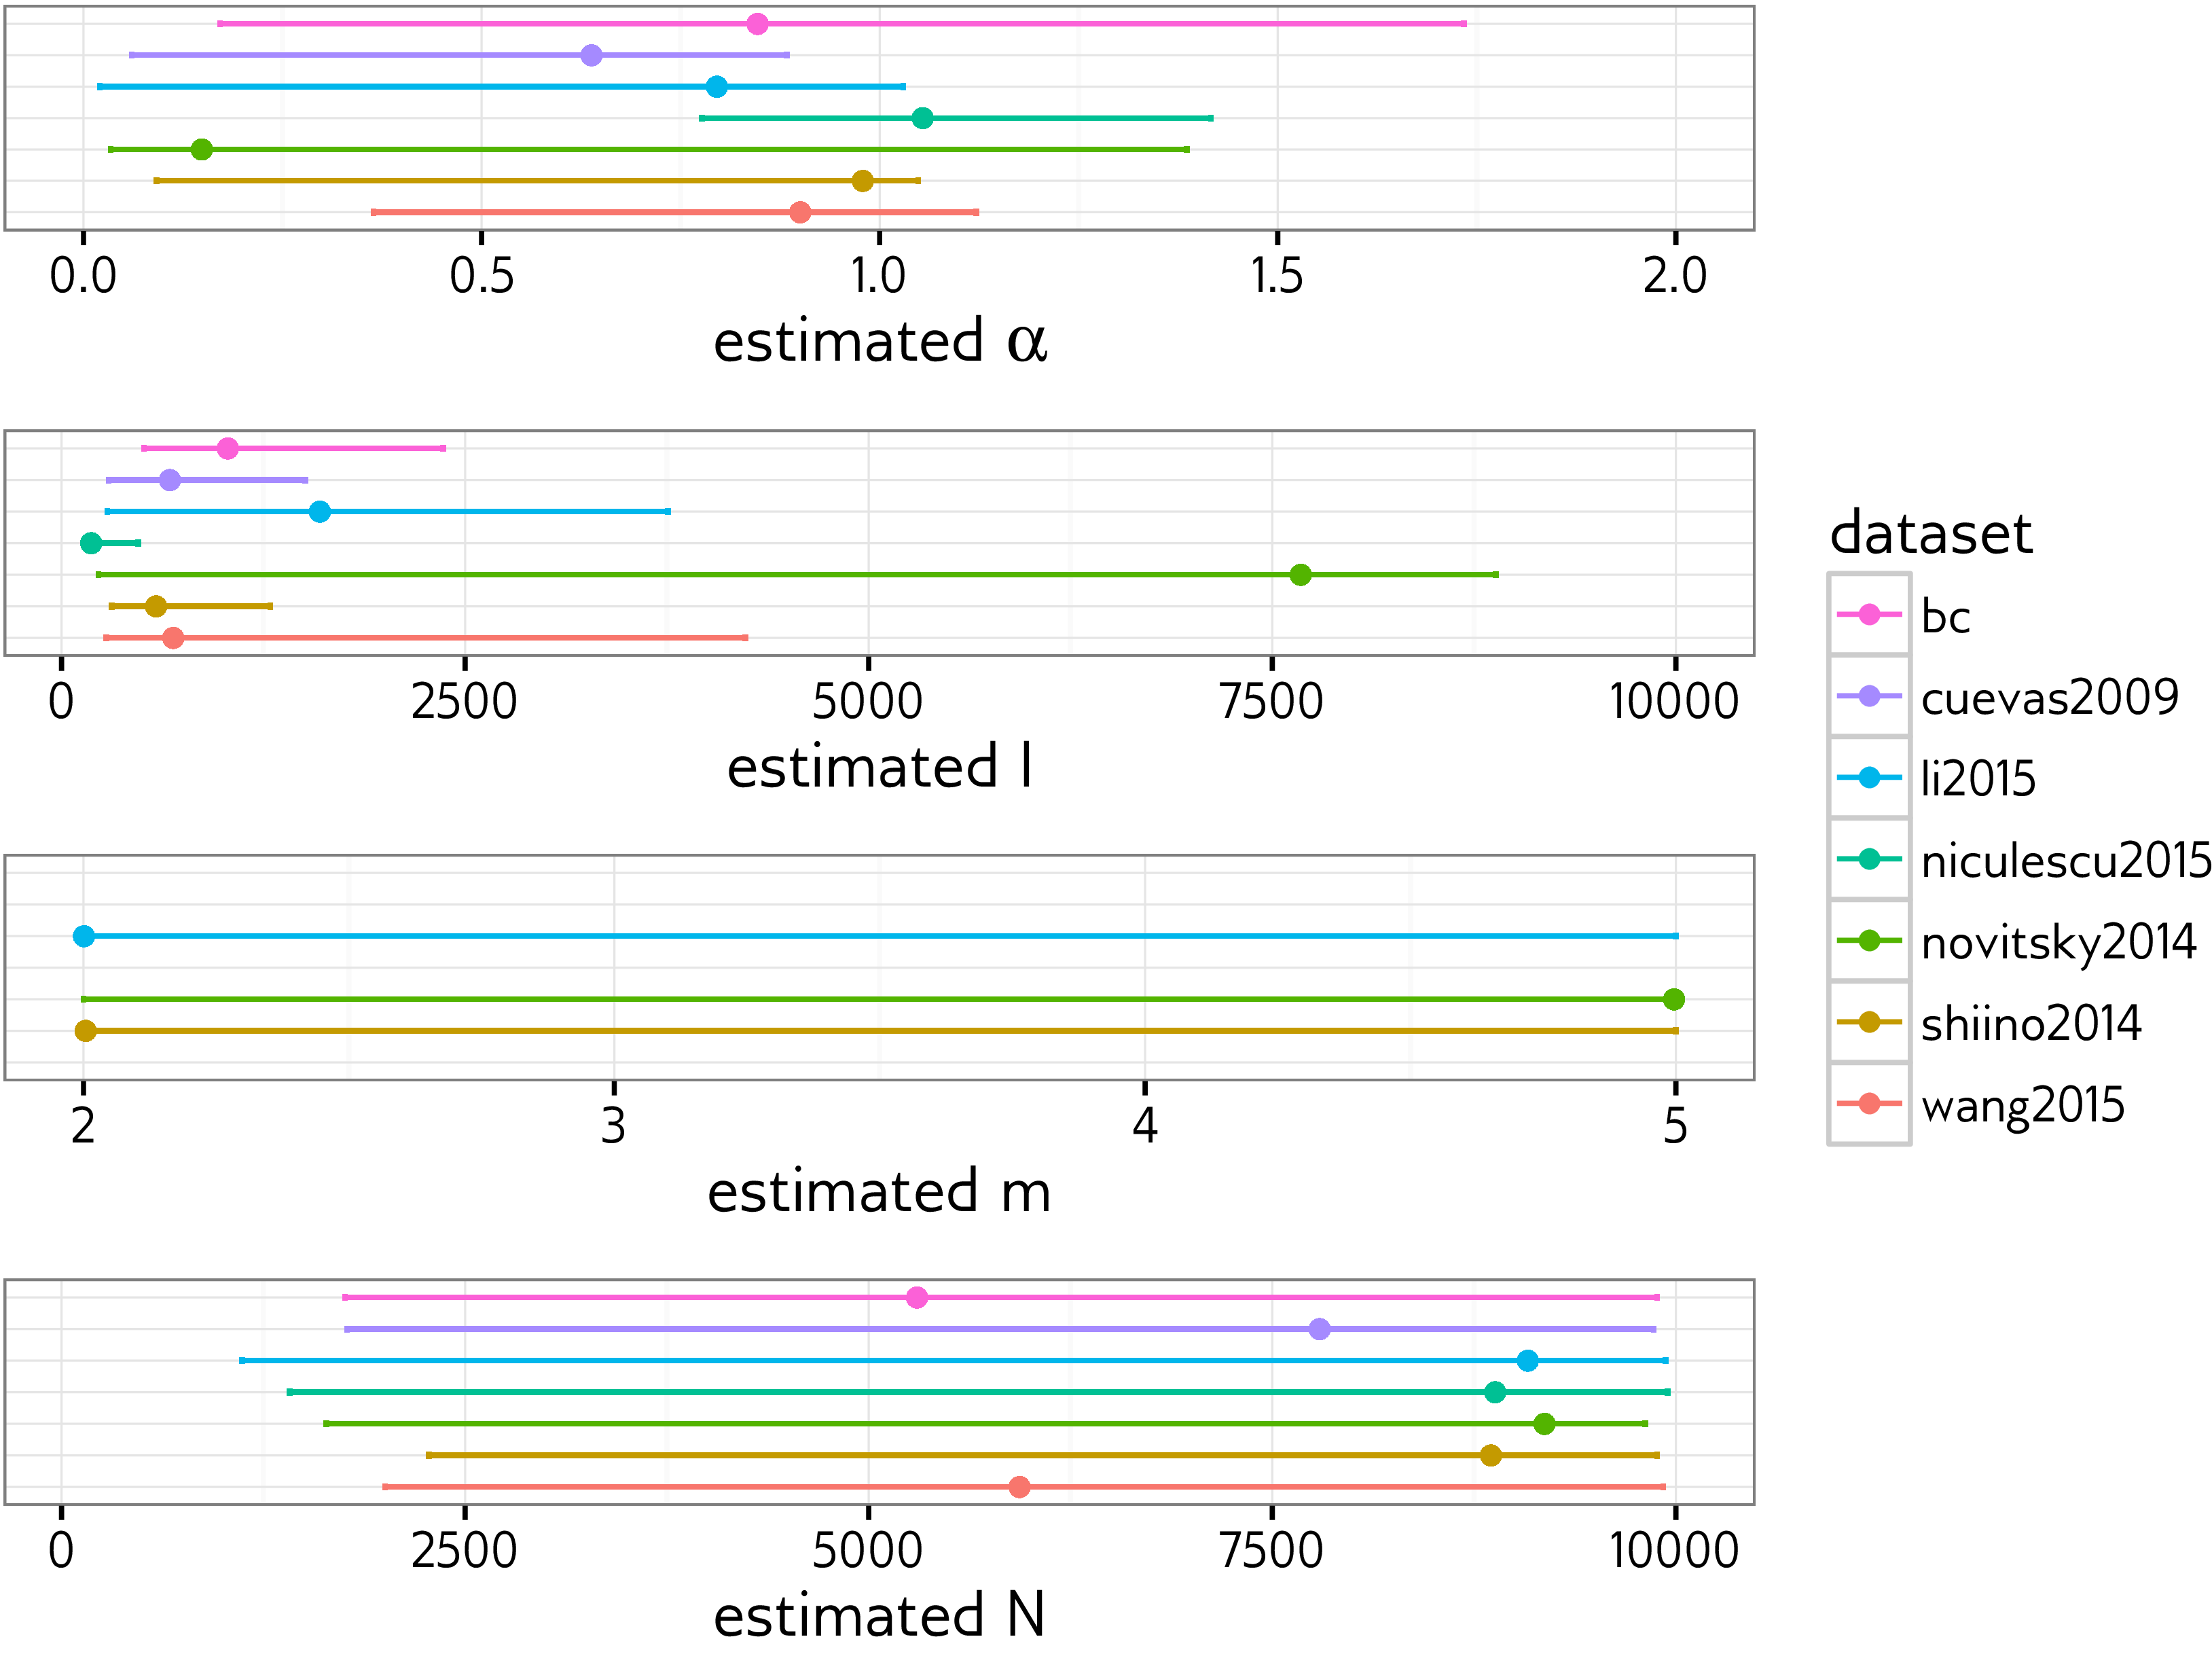
\includegraphics{realdata-hpd-bc}
  \caption[
      Maximum \textit{a posteriori} point estimates and 95\% HPD intervals for
      parameters of the BA network model, fitted to six HIV datasets
      with \software{netabc}.]
  {
      Maximum \textit{a posteriori} point estimates and 95\% HPD intervals for
      parameters of the BA network model, fitted to six HIV datasets with
      \software{netabc}. Legend labels indicate risk group and country of
      origin. Abbreviations: IDU, injection drug users; MSM, men who have sex
      with men; HET, heterosexual.
  }
  \label{fig:abchpd}
\end{figure*}

To make our analyses comparable to the existing network literature, we
estimated values of the power law exponent $\gamma$ for each of the datasets 
investigated. The results are summarized in \cref{tab:gamma}. All of the
estimated exponents were in the range $2 \leq \gamma \leq 2.5$, which is on the
lower end of the range $2 \leq \gamma \leq 4$ reported in the literature.

\begin{table}
    \centering
    % latex table generated in R 3.2.3 by xtable 1.8-2 package
% Mon Jun 20 11:25:36 2016
\begin{tabular}{lr}
  \hline
Dataset & $\gamma$ \\ 
  \hline
mixed/Spain (Cuevas et al. 2009) & 2.09 \\ 
  MSM/Shanghai (Li et al. 2015) & 2.10 \\ 
  MSM/USA (Little et al. 2014) & 2.10 \\ 
  MSM/Taiwan (Kao et al. 2011) & 2.42 \\ 
  MSM/Beijing (Wang et al. 2015) & 2.12 \\ 
  HET/Uganda (Grabowski et al. 2014) & 2.09 \\ 
  HET/Malawi (McCormack et al. 2002) & 2.32 \\ 
  HET/Botswana (Novitsky et al. 2013 \& 2014) & 2.44 \\ 
  IDU/Canada (unpublished) & 2.12 \\ 
  IDU/Romania (Niculescu et al. 2015) & 2.14 \\ 
  IDU/Estonia (Zetterberg et al. 2004) & 2.41 \\ 
   \hline
\end{tabular}

    \caption[
        Estimated power law exponents for six HIV datasets based on maximum
        \textit{a priori} estimates of BA model parameters.
    ]{
        Estimated power law exponents for six HIV datasets based on maximum
        \textit{a priori} estimates of BA model parameters. 100 networks were
        simulated using \textit{MAP} parameter estimates obtained with
        \software{netabc}. The power law exponent $\gamma$ was estimated for
        each, and the median of those estimates was used as a point estimate
        for the corresponding dataset.
    }
    \label{tab:gamma}
\end{table}


\chapter{Conclusion}

\printbibliography

\end{document}
